\chapter{Building Programs} % (fold)
\label{cha:building programs}

\begin{quote}
  \Fontlukas\Large
  \renewcommand{\LettrineTextFont}{\relax}
  \lettrine[image=true,lines=3,lraise=0.1]
  {M}{agic} requires both knowledge and tools. Our first lesson will uncover the tools of the Magi. Tools that you will need to use to practice magic. Here, take this ancient wand this orb and caldron. Each of these tools is essential to the working of even the most basic magic. Now lets see if you can wield that wand. Take it in your hand like this, and \ldots
\end{quote}

\bigskip

Software development requires both knowledge and tools. This first chapter will introduce you to the tools used by software developers. Tools that you will need to use to practice creating programs.

When you have understood the material in this chapter you will be able to make basic use of a Text Editor, the Terminal, and command line tools to create programs from source code. 

\minitoc

% =====================================
% = Concepts - Compilers and Programs =
% =====================================
\clearpage
\section{Concepts Related to Building Programs} % (fold)
\label{sec:concepts_related_to_building_programs}

In this chapter you will learn about the basic tools you need to use to create your own programs. You will see an example program, and then use these tools to convert that code into an executable program. You will then be able to run the program you created, and see it perform the tasks you coded.

This chapter provides a background on what programs are, and the general processes of how they are created. This will introduce you to the tools you will be using, and fill in some details of what they are doing and how to use them. The topics covered include the following:
\begin{itemize}
  \item \nameref{sub:what_is_a_program_}: This section introduces you to the idea of what a program is, and what it contains. You will need to be familiar with programs and what they are, as you will need to be able to create your own.
  \item \nameref{sub:machine_code}: Talks about the kinds of instructions the computer understands, and why it is not very productive to work at this level. You need to understand that this exists behind the scenes, but do not need to be overly familiar with it.
  \item \nameref{sub:assembly}: The next level of language is called Assembly. It is very close to machine code, but much easier to understand and use. However, this is still too low a level to be very productive. Just like machine code, you only need to know this exists
  \item \nameref{sub:source_code_and_the_compiler}: This is the level we are going to be working with in this book. This code is much easier to work with than assembly, and allows you to create your own programs reasonably quickly once you have learnt the basics. These are the tools you are going to be working with throughout this text.
  \item \nameref{sub:terminal}: This is a command line environment that lets you issue text commands to the user. You will use this to create and run your programs.
  \item \nameref{sub:hello world}: A \emph{classic} program used to check that you have everything working correctly. This section shows you the code that you can use this to check that you have all the tools setup correctly, and to check their usage.
  \item \nameref{sub:compiling_code}: This final section will show you how to use these tools to compile and run your own Hello World program. \fref{fig:run-1-helloworld} shows the Hello World program running from the Terminal.
\end{itemize}

\begin{figure}[b]
   \centering
   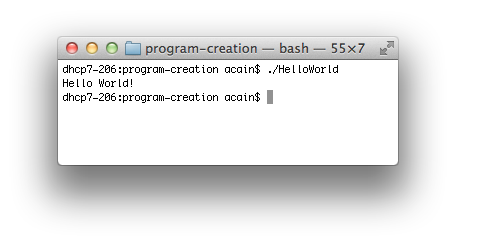
\includegraphics[width=0.7\textwidth]{./topics/programs-and-compilers/images/HelloWorld} 
   \caption{Hello World run from the Terminal}
   \label{fig:run-1-helloworld}
\end{figure}


\clearpage
\subsection{Programs} % (fold)
\label{sub:what_is_a_program_}

If you are going to learn to develop software you will need to become intimately aware of what a program is. After all, as a developer you will be creating your own programs.

A program is a file that contains instructions that get the computer to perform a task. Programs are lists of commands\footnote{C and Pascal are both \emph{imperative} programming languages. In the imperative paradigm a program is seen as a list of commands instructing the computer to perform actions.} telling the computer what to do, and the order in which to do it. Each instruction is very simple, but they can be executed very quickly, allowing computers to perform quite remarkable feats.

\begin{figure}[h]
   \centering
   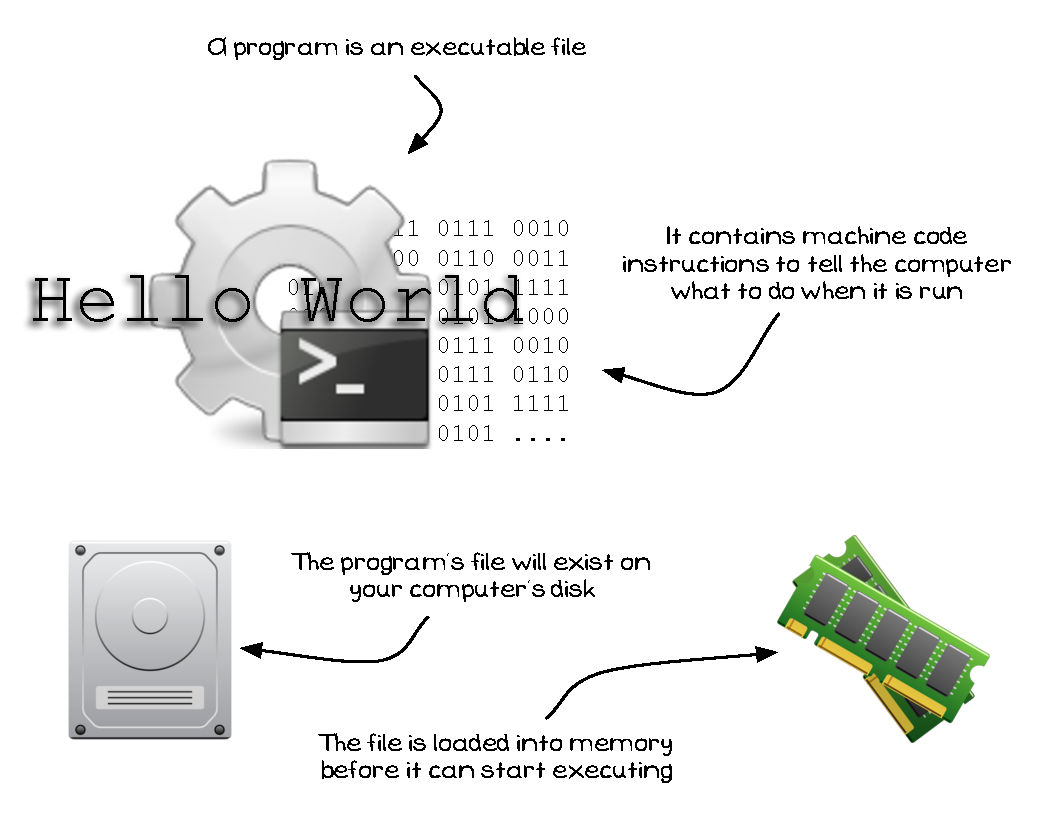
\includegraphics[width=0.9\textwidth]{./topics/programs-and-compilers/diagrams/Program} 
   \caption{A program contains instructions that command the computer to perform a task}
   \label{fig:what-is-a-program}
\end{figure}

\mynote{
\begin{itemize}
  \item You can \textbf{run} programs, which gets the computer to follow the instructions found within the program's file.
  \item To run, the program's instructions must first be loaded into memory.
  \item Once in memory, the computer starts running the instructions one after the other.
  \item When the last instruction is completed the program ends.
  \item There are several different ways to run a program:
  \begin{itemize}
    \item You can \emph{double-click} the program in a file browser.
    \item On tablets and app-phones you can \emph{tap} the program's icon.
    \item Advanced uses can enter \emph{text commands} in the Terminal to start programs.
  \end{itemize}
\end{itemize}
}

\clearpage
\subsubsection{What happens when a program runs?} % (fold)
\label{ssub:what_happens_when_a_program_runs_}

When you run a program, regardless of how it is started, the Operating System loads it from disk into memory and then starts it running. It is important that the file you try to run is a program. These are \emph{special} files that contain instructions the computer can understand.

\begin{figure}[h]
   \centering
   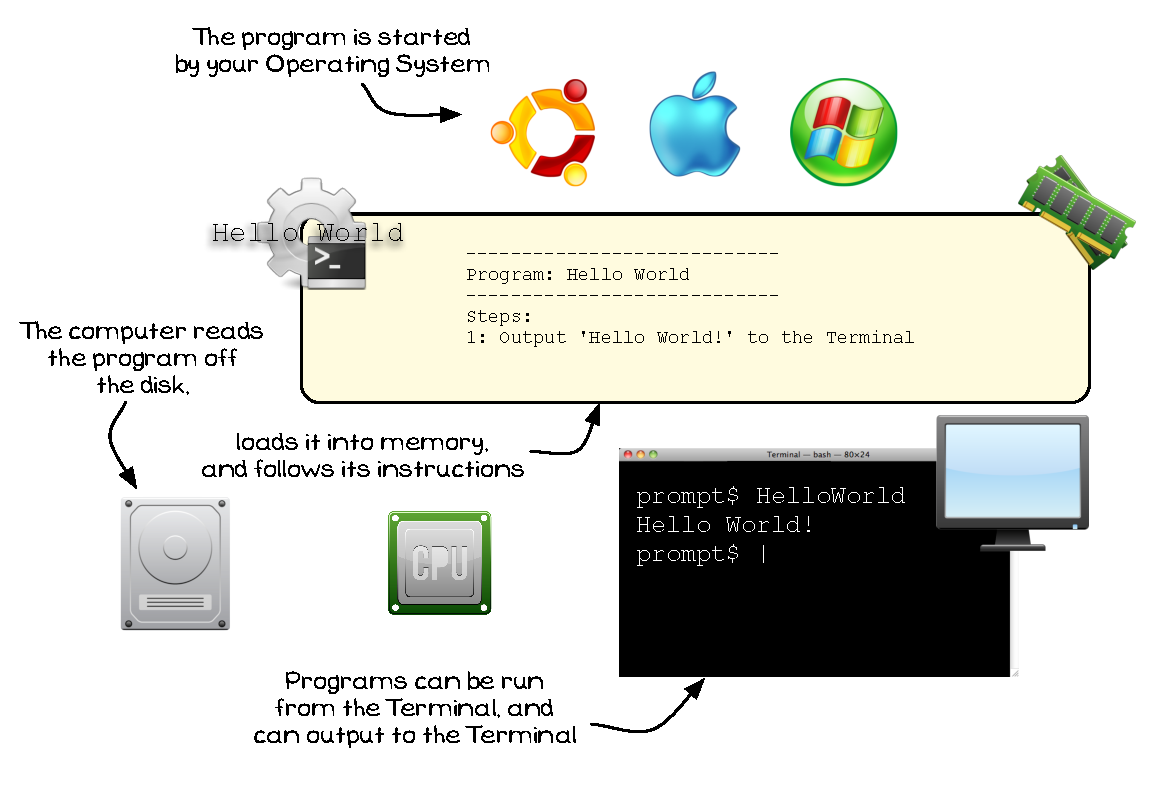
\includegraphics[width=0.9\textwidth]{./topics/programs-and-compilers/diagrams/ProgramExe} 
   \caption{Programs are loaded from disk into memory, then run}
   \label{fig:what-is-a-program-exe}
\end{figure}

\mynote{
\begin{itemize}
  \item Your Operating System is a piece of software that is responsible for managing your computer's hardware.
  \item One of the Operating System's responsible is to start programs.
  \item The \nameref{sub:terminal} can be used to start programs.
  \item Programs can also output to the Terminal.
  \item A Program must contain instructions that the computer can understand.
\end{itemize}
}

% subsubsection what_happens_when_a_program_runs_ (end)

% subsection what_is_a_program_ (end)
\clearpage
\subsection{Machine Code} % (fold)
\label{sub:machine_code}

\emph{What instructions do Computers understand?}

Computers do not really \emph{understand} anything, computers are \textbf{unintelligent}. They are a machine that respond in a set way to a given number of instructions. The instructions that a computer uses is called its {\em instruction set} and contain instructions to perform basic mathematic operations, loading and storing data in memory, comparing numeric values, and moving to the new instruction elsewhere in the program. These very simple actions are performed very quickly, and can be use to create everything you have ever seen a computer do.

The computers instructions can be seen as binary numbers, numbers made from 0's and 1's. These values are like switches that are either off (0) or on (1). Setting these \emph{switches} to different sequences will cause the computer to perform different actions. For example, the \emph{switch} combination \texttt{0000 0011}, may cause the computer to add two numbers together. Any time you want the computer to perform this task you set the switches to that combination. These binary instructions are called \textbf{machine code}.

\begin{figure}[h]
   \centering
   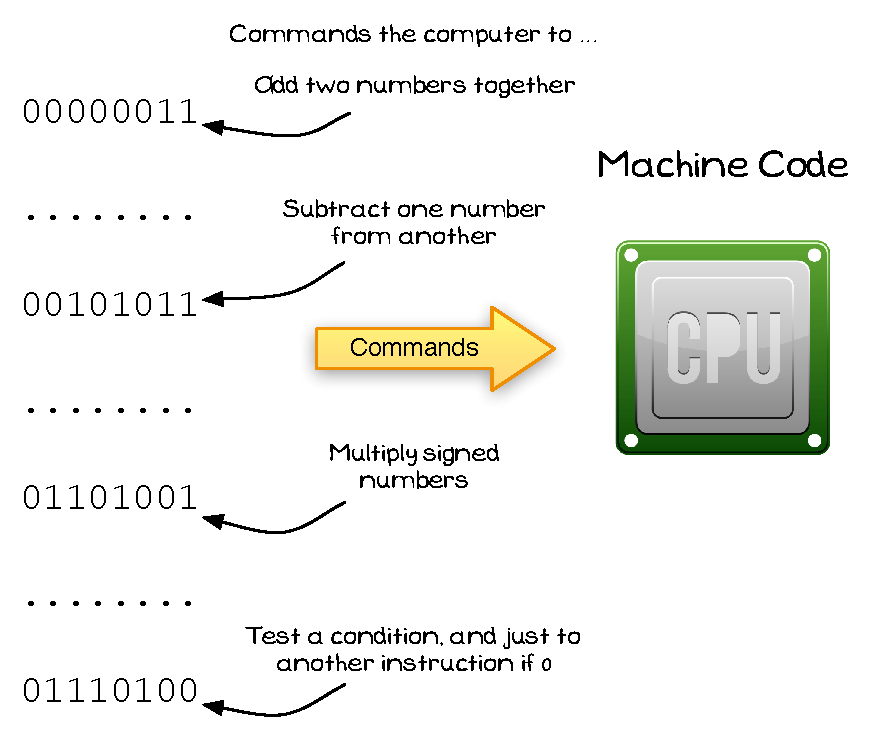
\includegraphics[width=0.8\textwidth]{./topics/programs-and-compilers/diagrams/MachineCode} 
   \caption{The computer responds to machine code instructions}
   \label{fig:machine-code}
\end{figure}

\mynote{
\begin{itemize}
  \item The \textbf{CPU}, Central Processing Unit, is the workhorse of the computer. It executes the program's instructions.
  \item The instructions a CPU uses is called its \textbf{Instruction Set}, and different CPUs have different instruction sets.
  \item Some common instruction sets: ARM (used in iPhones and iPads), x86-64 (used in desktops), and PowerPC (used in the XBox360 and Playstation 3). 
\end{itemize}
}

\clearpage

\subsubsection{Programming in Machine Code} % (fold)
\label{ssub:programming_in_machine_code}

Listing \ref{lst:machine code} shows a chunk of the machine code for a small program. These 1s and 0s are the codes used to instruct the computer when this program is executed. Programs can be written directly in machine code, but this is a time consuming task. This is further complicated by the fact that machine code is unique to each kind of CPU. This means that programming at this level is entirely dependent on the kind of processor that you are targeting.

\begin{lstlisting}[caption={128 bits from the 106,752 bits of Machine Code from a small program.},label={lst:machine code}]
...
0110 0111 0111 0010 0000 0000 0110 0011 0100 1110 0101 1111 0100 0001 0101 1000
0110 0111 0111 0010 0000 0000 0111 0110 0101 1111 0101 1111 0110 1001 0101 1111
...
\end{lstlisting}

No one wants to have to work at this level of details, and fortunately you do not need to. Software developers have created tools to help them create programs without having to think about these low level details. These tools make it possible to work at a \textbf{higher level of abstraction}. They take the code you write, and do the hard work of converting that to the machine code of the computer you want to run it on.

\mynote{
\begin{itemize}
  \item You can look at the machine code of any program on your computer. You just need the right tools.
  \item If you open the program's executable file in a text editor it will look very strange, and not at all like a large list of binary values. This is because the text editor displays one character for every byte (or two bytes depending on the file) from the file.
  \item A \textbf{Hex Editor} is a program that is useful for examining binary data. It shows you one character for every four bits in the file.
\end{itemize}
}

\begin{table}[h]
  \ttfamily
  \centering
\begin{tabular}{|c|c||c|c||c|c||c|c|}
  \hline
  Binary & Hex & Binary & Hex & Binary & Hex & Binary & Hex  \\
  \hline
  0000 & \textbf{0} & 0001  & \textbf{1}  & 0010  &  \textbf{2} & 0011 & \textbf{3} \\
  0100 & \textbf{4} & 0101 & \textbf{5} & 0110 & \textbf{6} & 0111 & \textbf{7} \\
  1000 & \textbf{8} & 1001 & \textbf{9} & 1010 & \textbf{A} & 1011 & \textbf{B} \\
  1100 & \textbf{C} & 1101 & \textbf{D} & 1110 & \textbf{E} & 1111 & \textbf{F} \\
  \hline
\end{tabular}
  \caption{Binary to Hexadecimal}
\end{table}

\begin{figure}[h]
   \centering
   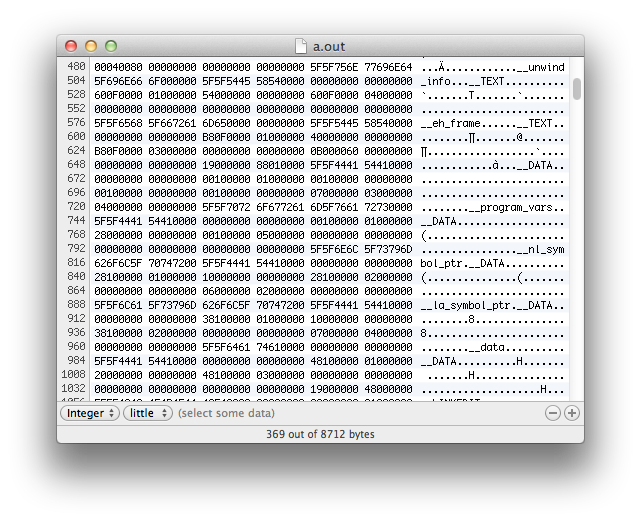
\includegraphics[width=0.55\textwidth]{./topics/programs-and-compilers/images/HexEditor} 
   \caption{A HexEditor allows you to view the machine code of any program}
   \label{fig:hex-editor}
\end{figure}


% subsubsection programming_in_machine_code (end)

% subsection machine_code (end)
\clearpage
\subsection{Assembly} % (fold)
\label{sub:assembly}

The next level of abstraction up from machine code is called \textbf{Assembly}, or \textbf{Assembler Code}. Here the numeric machine code instructions are given symbolic names that are, to some degree, more understandable for humans. The code \texttt{0000 0011} may be given the symbolic name \texttt{add}, for example.

Programs written in this language cannot be executed directly by the computer, it isn't machine code. Assembler code is converted to machine code by a program called an \textbf{Assembler}. This program reads the instructions from the assembler code and outputs machine code. So, for example, anywhere it encounters \texttt{add} in the code it can output \texttt{0000 0011}.

\begin{figure}[h]
   \centering
   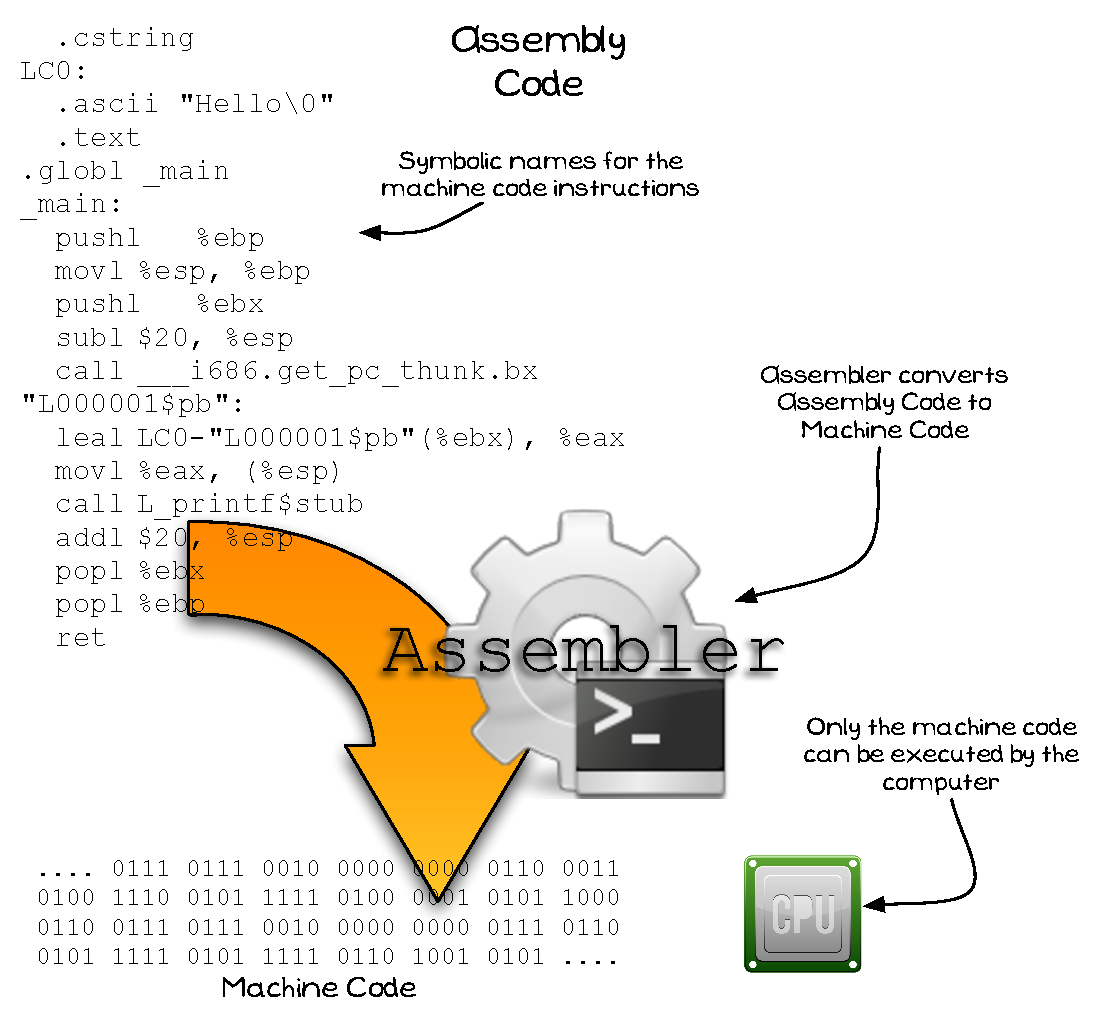
\includegraphics[width=0.8\textwidth]{./topics/programs-and-compilers/diagrams/Assembly} 
   \caption{The computer responds to machine code instructions}
   \label{fig:assembly}
\end{figure}

\mynote{
\begin{itemize}
  \item As with \nameref{sub:machine_code}, Assembly is liked to individual CPUs.
  \item Assembly is very close to Machine Code, its machine code with symbolic names for the instructions.
\end{itemize}
}

\clearpage
\subsubsection{Programming in Assembly} % (fold)
\label{ssub:programming_in_assembly}

The code in Listing \vref{asmcode} shows an example of some assembler code. This is the assembler code that was used to generate the machine code from Listing \ref{lst:machine code}. The machine code was 13,344 bytes in size, where the same program in assembler code is only 658 bytes. The assembler reads these 658 bytes, combines it with instructions from program libraries, and outputs machine code. 
\lstset{language=[x86masm]{assembler}}

\begin{lstlisting}[caption={Assembler Sample},label={asmcode}]
  .cstring
LC0:
  .ascii "Hello\0"
  .text
.globl _main
_main:
  pushl	%ebp
  movl	%esp, %ebp
  pushl	%ebx
  subl	$20, %esp
  call	___i686.get_pc_thunk.bx 
"L000001$pb":
  leal	LC0-"L000001$pb"(%ebx), %eax
  movl	%eax, (%esp)
  call	L_write_line$stub
  addl	$20, %esp
  popl	%ebx
  popl	%ebp
  ret
\end{lstlisting}

From a programmer's perspective, assembler code is much easier to work with than machine code, though there are still issues with the use of assembler code. Firstly Assembly is bound to the instruction set of the CPU that you are targeting, meaning that if you want to support other kinds of CPU you will need to rewrite the program. The other main issue with assembler code is that while it is more understandable, you are still working with the primitive instructions of the CPU. Working at this level takes considerable effort to write even simple programs.

Assembly languages were first developed in the 1950s, and were known as a \textbf{Second Generation}\footnote{First Generation being Machine Code.} programming languages. This step forward did make programming easier, but the tools have advanced since then and now we can work at an even higher level of abstraction.

% subsubsection programming_in_assembly (end)

% subsection assembly (end)
\clearpage
\subsection{Source Code and the Compiler} % (fold)
\label{sub:source_code_and_the_compiler}

The next step in programming language evolution moved from machine level instructions to something more human readable. These languages, known as \textbf{Third Generation Languages}, use move advanced programs than assemblers to convert their instructions into machine code. Programs written in these languages have their code converted to machine code by a \textbf{compiler}.

A \textbf{Compiler} is a program that converts \textbf{Source Code} into machine code that is saved into an executable file called a \emph{Program}. The program can then be executed independent of the compiler and the source code.

Internally, a compiler will perform a number of steps, as shown in \fref{fig:compiler}.

\begin{enumerate}
  \item \textbf{Preprocessing}: The code is read from your source code files. This may involve some processing of the text itself, which includes things like ignoring any comments in the code.
  \item \textbf{Compiling}: The code is then converted into assembly instructions, and an assembly program is output.
  \item \textbf{Assembling}: The assembly version of the program is converted into machine code, and stored in \textbf{object files}.
  \item \textbf{Linking}: In the final step the compiler uses a \textbf{Linker} to join together the machine code from your program, with other machine code you have used from the programming libraries. This then outputs an executable program.
\end{enumerate}

\begin{figure}[h]
   \centering
   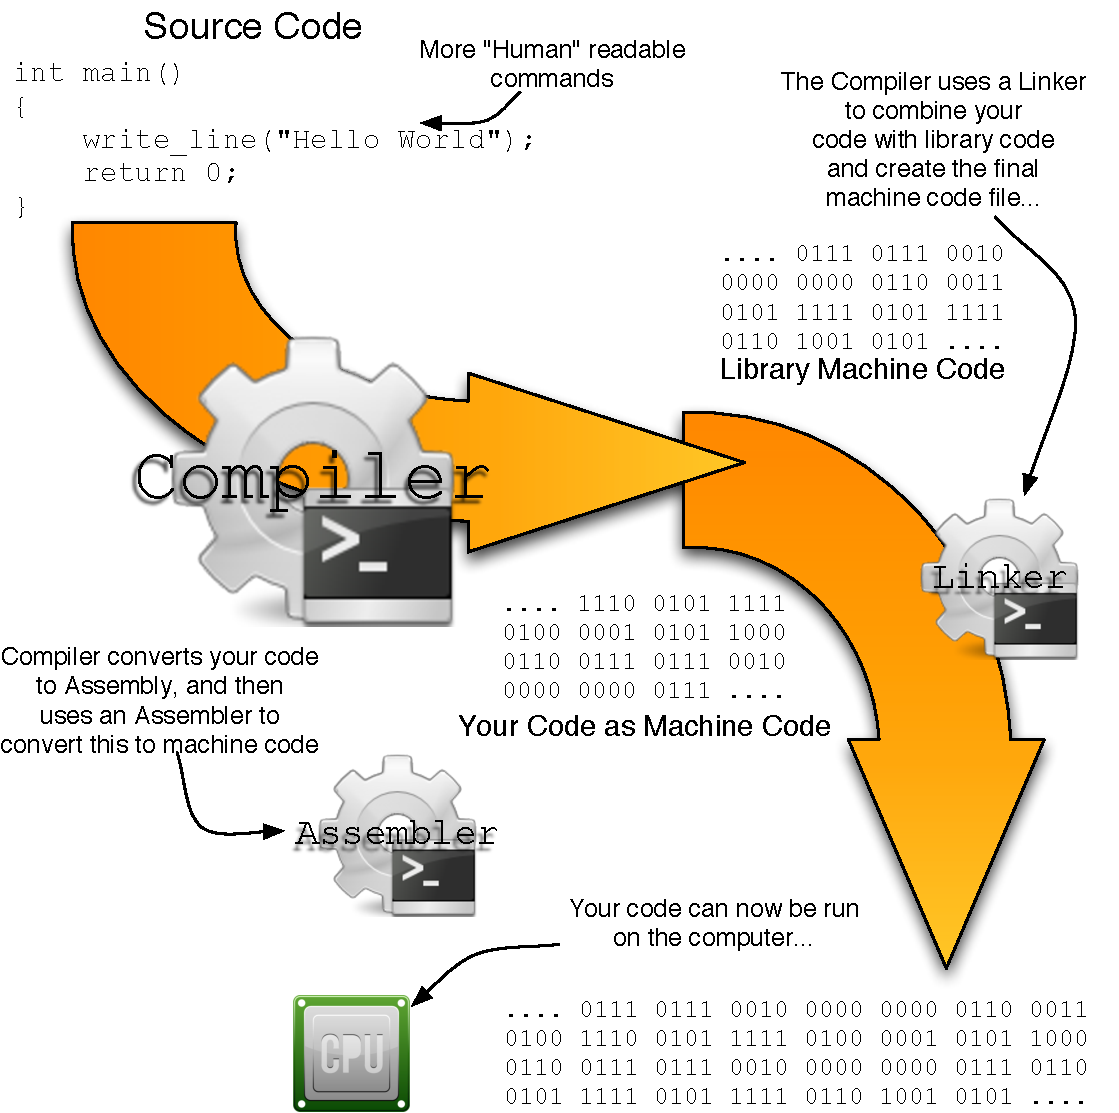
\includegraphics[width=0.8\textwidth]{./topics/programs-and-compilers/diagrams/Compiler} 
   \caption{Compilers turn Source Code into Machine Code}
   \label{fig:compiler}
\end{figure}

\clearpage
\subsubsection{Programming with a Third Generation Language} % (fold)
\label{ssub:programming_with_a_third_generation_language}

\lref{lst:hello-world-c-1} and \lref{lst:hello-world-pas-1} show two examples of source code. This code describes a small program that can be used to output a message to the \nameref{sub:terminal}.

\begin{multicols}{2}
  \ccode{lst:hello-world-c-1}{Example C code}{code/c/program-creation/hello-world.c}
  \columnbreak
  \pascode{lst:hello-world-pas-1}{Example Pascal code}{./topics/program-creation/pascal/HelloWorld.pas}
\end{multicols}

The code shown in \lref{lst:hello-world-c-1} shows the code for the C program that was used to generate the assembler code, and machine code shown in the previous code listings. This code must be converted by the C compiler into machine code before it can be run. It is interesting to note the size of the C file: it is only 50 bytes! The compiler converts this 50 bytes into the 13,344 bytes of machine code. 

\lref{lst:hello-world-pas-1} shows the same program written in the Pascal programming language. Like its equivalent C code, this must be compiled to create a program you can run.

Programs written in a third generation programming language are much easier to understand than their assembler or machine code counterparts. It is also possible that this code can be compiled to run on different types of CPU, making it more portable. Most modern programming languages are third generation programming languages.


The code that a programmer writes in these languages is called \textbf{Source Code}. Typically source code is saved into a text file with a file extension that helps identify the language it is written in. For example, programs written in the C language are saved into files with a {\tt .c} file extension whereas Pascal programs are saved into files with a {\tt .pas} extension.

\mynote{
\begin{itemize}
  \item There are may different Third Generation Languages, including both C and Pascal.
  \item Each language has its own compiler that understands that language's code.
  \item The C compiler we will use is called \textbf{gcc} - this stands for \textbf{GNU C Compiler}.
  \item The Pascal compiler we will use is called \textbf{fpc} - this stands for \textbf{Free Pascal Compiler}.
\end{itemize}
}



% subsubsection programming_with_a_third_generation_language (end)

% subsection source_code_and_the_compiler (end)
% \clearpage
\subsection{Challenges and Rewards} % (fold)
\label{sub:challenges_and_rewards}

% subsection challenges_and_rewards (end)

Programming in a third generation language, like C++ and Pascal, requires you to master several different things, as shown in the following list. The following chapters will work on building your knowledge and skills in each of these aspects.

\begin{enumerate}
  \item What is it that you want the program to do? Writing a program is like writing instructions for someone to carry out. If you do not know how to perform the task yourself you will not be able to tell someone else how to perform the task.
  \item You need to understand what the computer is capable of doing. Computers are unintelligent, so writing a program is more challenging than giving instructions to a person as the computer cannot interpret what you mean and will follow your instructions to the letter, regardless of the effect. The capabilities of the computer limit the flexibility you have for expressing your solution.
  \item The language you choose to develop with also limits how you express your solution. You need to understand the artefacts that you can create, how these artefacts are written in source code, and how these are executed by the computer.
  \item Finally you need to understand how to locate and correct issues with your programs. This includes responding to syntax errors reported to you by the compiler, as well being able to locate errors where the program does not operate the way you intended. 
\end{enumerate}

\emph{With all of these challenges, what appeal does software development have?}

There is nothing better than seeing a program you created running on a computer. You have brought the machine to life, getting it to perform a task the way you want it performed. Once you get a program working it can become easy to get hooked and working on new features and functions becomes a real joy. The greater the challenge the program offers, the greater your sense of achievement when you see the working product in operation.

% subsection compiling_code (end)
\clearpage
\subsection{Terminal} % (fold)
\label{sub:terminal}

Once you have written some source code, you need to be able to compile it. This means, you need to run the \textbf{compiler}, and give it your source code files to compile. The best way to do this when you really want to learn about programming, is to run the compiler directly yourself. To do this you needed to use a \textbf{Terminal} program.

The Terminal is a program that gives you command line access to the computer. With command line access you can enter text commands to start programs. These programs can output details back to the Terminal for you to read, and interactive programs can also read input from you via this same Terminal.

\begin{figure}[h]
   \centering
   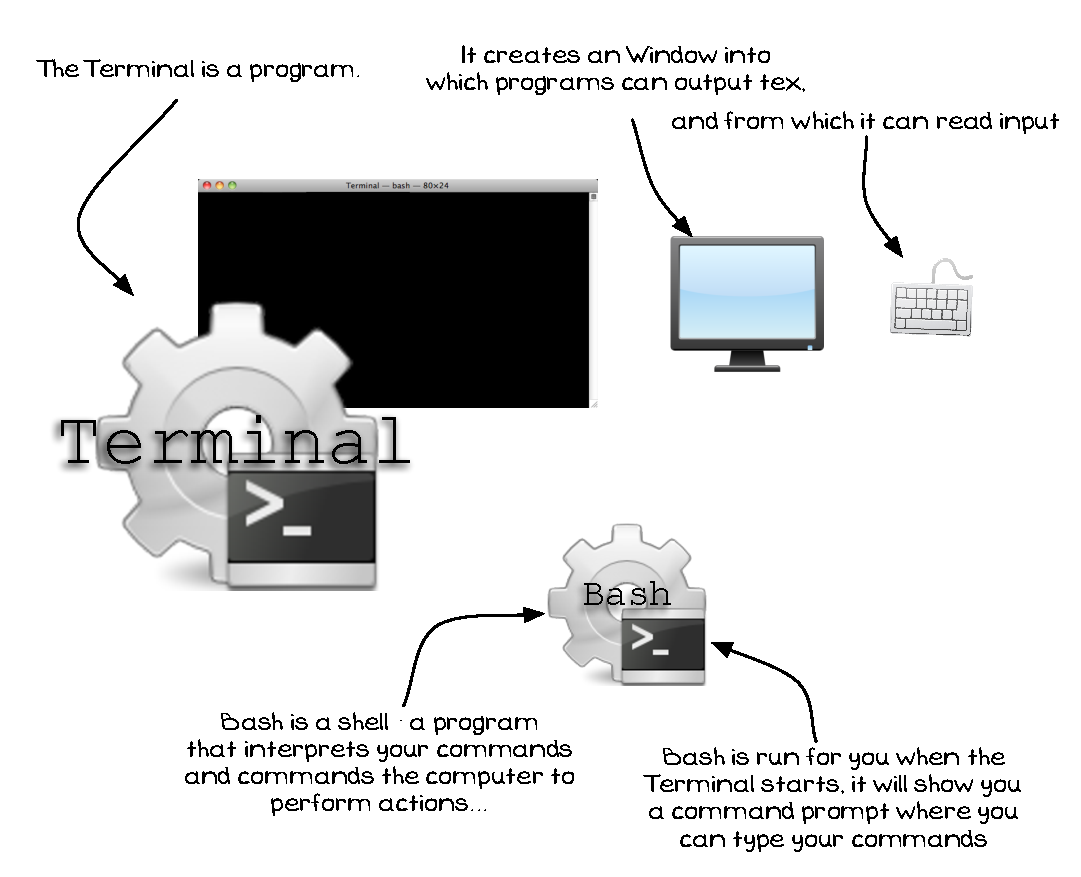
\includegraphics[width=0.8\textwidth]{./topics/programs-and-compilers/diagrams/Terminal} 
   \caption{The Terminal program gives you command line access to your computer}
   \label{fig:terminal}
\end{figure}

\mynote{
\begin{itemize}
  \item On Ubuntu \textbf{Linux} you can find the Terminal in the \emph{Accessories} folder within \emph{Applications}. See Figure \ref{fig:program-creation-ubuntu-terminal}.
  \item On \textbf{MacOS} you can find the Terminal in the \emph{Utilities} folder within \emph{Applications}. See Figure \ref{fig:program-creation-macos-terminal}.
  \item On \textbf{Windows} you will need to download and install \emph{MSys2}. The \emph{MSys2 Shell} is the equivalent of Terminal on the other operating systems. The details for how to install this are in the SplashKit installation guides.

  \item The Terminal is also be called the \textbf{console} or \textbf{command prompt}.
\end{itemize}
}

\clearpage
\subsubsection{The Shell} % (fold)
\label{ssub:the_shell}

The \textbf{Terminal} program itself just provides a text environment, allowing text input and output. Within this environment a \textbf{Shell} program is run to interpret your commands. This is an interactive program that will display a prompt to you, at which you enter your commands.

There are a number of different Shell programs, each of which has its own set of instructions. The Shell we are going to use in this book is called \textbf{Bash}. This shell program is available on Linux, Mac OS, and Windows. As a Unix shell it is native for Linux and Mac OS, and with Windows you can install \textbf{MSys2} to use these commands.

\begin{figure}[h]
   \centering
   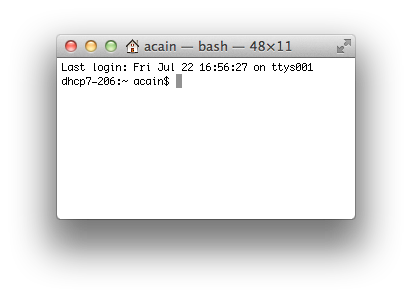
\includegraphics[width=0.6\textwidth]{./topics/programs-and-compilers/images/Bash} 
   \caption{The Terminal running Bash}
   \label{fig:bash}
\end{figure}

A shell program is very simple. It provides a text prompt at which you can enter commands. The Shell then reads the text you entered, and performs an action based on the text you entered. You can use the Shell to perform operations like copying and deleting files, and starting programs.

\mynote{
\begin{itemize}
  \item The name `Shell' came from idea that this was the outermost \emph{shell} of the computer, the interface between the user and the computer's internals.
  \item Bash stands for `\emph{Bourne-again shell}', as Bash is a replacement for the \emph{Bourne} shell.
  \item It will take some time to get used to using Bash, but the more you learn about it the more useful it will become.
\end{itemize}
}

% subsubsection the_shell (end)
\clearpage
\subsubsection{Using Bash} % (fold)
\label{ssub:bash}

To get started using Terminal you will need to know some Bash commands, see \tref{tbl:bash-commands}.

\begin{table}[h]
  \centering
  \begin{tabular}{|l|l|p{5cm}|}
    \hline
    \textbf{Action} & \textbf{Command} & \textbf{Description} \\
    \hline
    Change Directory & \texttt{cd} & Moves the shell to a different working directory. \\
    \hline
    Print Working Directory & \texttt{pwd} & Outputs the current working directory.\\
    \hline
    List Files & \texttt{ls} & Outputs a list of files.\\
    \hline
    Copy File(s) & \texttt{cp} & Copies files from one location to another.\\
    \hline
    Move File(s) & \texttt{mv} & Moves files from one location to another.\\
    \hline
    Delete File(s) & \texttt{rm} & Removes files from the computer. There is no recycle bin with this, so take care!\\
    \hline
    Create a Directory & \texttt{mkdir} & Makes a new directory. \\
    \hline
  \end{tabular}
  \caption{Some bash commands to get you started}
  \label{tbl:bash-commands}
\end{table}

To get started with Bash, you need to understand a little bit about the \textbf{file system}. Each operating system needs a way of storing its files, and there are going to be lots of files stored on a computer. This means that it would be cumbersome to try and keep these all in one place. Instead, the Operating System places files in \textbf{directories} (also known as \emph{Folders}). A directory can contain files, and other directories. 

When you are working in Bash, you will have a \textbf{working directory}. This is the directory where Bash will start searching for the files you are interacting with. To start working with the compiler you will need to be able to use the \textbf{change directory} command to move to the directory that contains your source code files.

With the \textbf{Change Directory} command you tell Bash which directory you want to move into, with the different parts of this path being separated by forward slashes (/). Example commands to move to your Documents directory are shown in \tref{tbl:dirs}, with screenshots for Linux in \fref{fig:linux-files}, Mac OS in \fref{fig:mac-files}, and Windows in \fref{fig:win-files}.

\begin{table}[h]
  \centering
  \begin{tabular}{|l|l|}
  \hline
  \textbf{Operating System} & \textbf{CD Command}  \\
  \hline
  \emph{Linux} & \texttt{cd /home/\emph{uname}/Documents} \\
  or & \texttt{cd $\sim$/Documents} \\
  \hline
  \emph{Mac OS} & \texttt{cd /Users/\emph{uname}/Documents} \\
  or & \texttt{cd $\sim$/Documents} \\
  \hline
  \emph{Windows} & \texttt{cd /c/Users/\emph{uname}/Documents} \\
  \hline
\end{tabular}
  \caption{CD command to move into your documents directory on various Operating Systems. In these examples \texttt{\emph{uname}} should be replaced by your user name. The examples in \fref{fig:linux-files}, \fref{fig:mac-files}, and \fref{fig:win-files} are for the user \texttt{acain}.}
  \label{tbl:dirs}
\end{table}

\mynote{
\begin{itemize}
  \item You can find many resources on using Bash on the web, a fairly extensive overview of these commands can be found at \url{https://dev.to/awwsmm/101-bash-commands-and-tips-for-beginners-to-experts-30je}.
  \item After you run the \texttt{cd} command, you can check which directory you are in using the \textbf{pwd} command. To do this just type \texttt{pwd} and press enter.
  \item Once you get used to the \texttt{cd} command you can start exploring the other commands.
\end{itemize}
}

\begin{figure}[p]
   \centering
   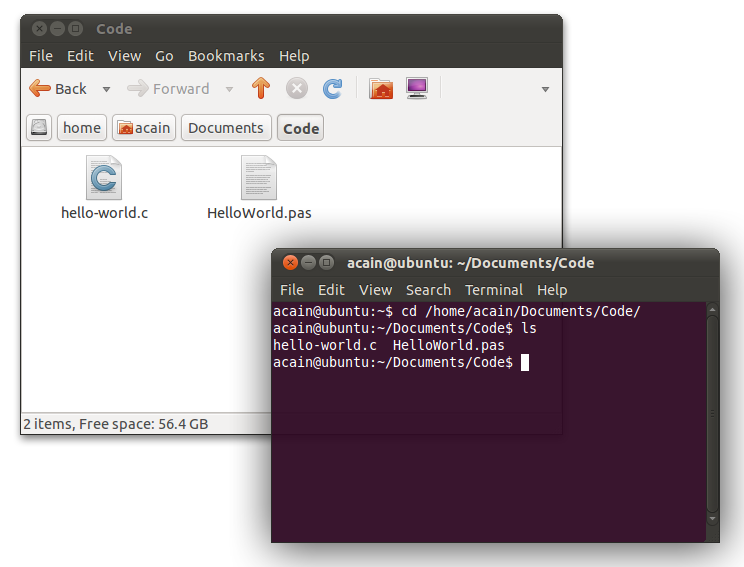
\includegraphics[width=0.9\textwidth]{./topics/programs-and-compilers/images/LinuxFiles} 
   \caption{Changing directories in Linux (Ubuntu)}
   \label{fig:linux-files}
\end{figure}

\begin{figure}[p]
   \centering
   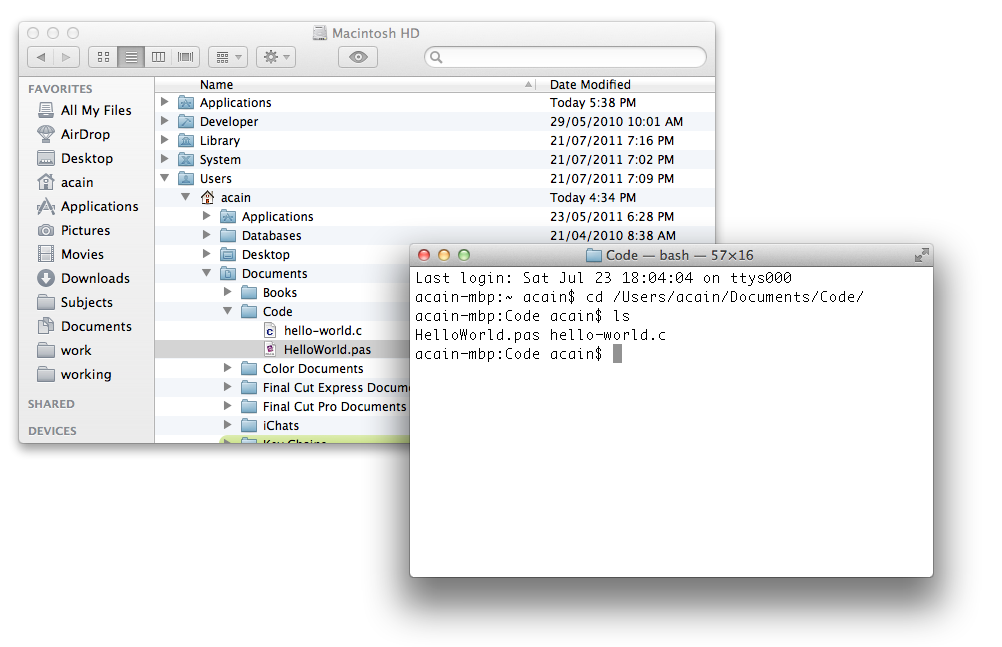
\includegraphics[width=0.9\textwidth]{./topics/programs-and-compilers/images/MacFiles} 
   \caption{Changing directories in MacOS}
   \label{fig:mac-files}
\end{figure}


\begin{figure}[p]
   \centering
   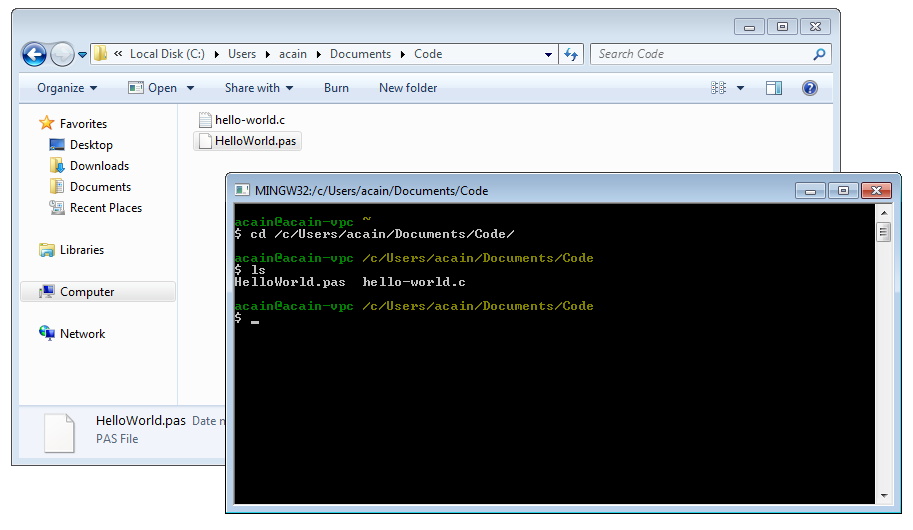
\includegraphics[width=\textwidth]{./topics/programs-and-compilers/images/WindowsFiles} 
   \caption{Changing directories in Windows}
   \label{fig:win-files}
\end{figure}



% subsubsection bash (end)

% subsection terminal (end)
\clearpage
\subsection{The First Program: Hello World} % (fold)
\label{sub:hello world}

There is one very special program that all developers create. This is the first program a software developer creates when they start using a new language, or technology. It is the famous \textbf{Hello World}!

This is a very simple program, it runs and outputs the text `Hello World' to the Terminal. So, why is this the first program? It makes sure that everything is set up correctly. If `Hello World' does not work, then there is something wrong with your setup you need to check.

Listings \ref{lst:hello-world-c} and \ref{lst:hello-world-pas} show the code for the `Hello World' program written with the C++ and Pascal programming languages. Both programs result in the same output when run: they write the text `Hello World!' to the Terminal. They both use the same basic programming structures, and they both go about performing the task in the same way. At this stage, however, they are both just fancy text. What we need to do is use a special tool to convert these into \emph{programs}, we need to \textbf{compile} them.

\csection
{
\ccode{lst:hello-world-c}{Hello World code in C++.}{code/c/program-creation/hello-world.c}
}

\passection{
 \pascode{lst:hello-world-pas}{Hello World code in Pascal.}{./topics/program-creation/pascal/HelloWorld.pas}
}

\mynote{
\begin{itemize}
  \item This source code needs to be written into a \textbf{text file}.
  \item C++ source code usually has a \textbf{.cpp} file extension. For example, \textbf{hello-world.cpp}.
  \item Pascal source code usually has a \textbf{.pas} file extension. For example \textbf{HelloWorld.pas}.
  \item It is a good idea to create a directory (folder) under which you will place your code. Within this directory you can create other directories for individual projects, or for the code related to the chapters in this book.
\end{itemize}
}

% section hello world (end)

\input{topics/programs-and-compilers/concepts/Summary}


% section concepts_related_to_building_programs (end)

% ========================
% = Using these concepts =
% ========================

\clearpage
\section{Using these concepts: Compiling a Program} % (fold)
\label{sec:using_these_concepts_compiling_a_program}

Now that the concepts have been presented, let us have a look at how these can be used to create a program. We will take the code from the Hello World, and use a compiler to turn this code into a program that we can then execute. This process is the same for large and small programs.

\subsection{The SplashKit Manager: skm} % (fold)
\label{sub:skm}

Before we get started, there is one additional tool that we can use to help make SplashKit programs easier to work with: the SplashKit Manager (\textbf{skm}). `skm' is a command line tool that comes with SplashKit when you install it. It is designed to take your compiler instructions, and add the extra options needed to link with the SplashKit library.

The best way to get started with a SplashKit program is to create a new folder (directory) in your file system that will be used to store the code and other files related to that program. 

\csection{
The following commands create a \emph{MyProject} folder, setup a new C++ project, and then compile it into a program.

\bashcode{lst:c-create-project}{Creating a C++ project with skm.}{code/c/program-creation/create-cpp-project.sh}
}

\passection{
The following commands create a \emph{MyProject} folder, setup a new Pascal project, and then compile it into a program.

\bashcode{lst:pas-create-project}{Creating a Pascal project with skm.}{code/pascal/program-creation/create-fpc-project.sh}
}

\subsection{Making the Hello World Program} % (fold)
\label{sub:compiling_code}

\lref{lst:hello-world-c} and \lref{lst:hello-world-pas} show the source code for the Hello World program. To make this into a program you need to:

\begin{enumerate}
  \item Write the code into a text file.
  \item Save the text file to disk.
  \item Compile it.
\end{enumerate}

Step 1 and 2 can be accomplished with any text editor, but the best ones to use highlight your code. Each programming language has rules that determine how its code must be formatted. This is known as the language's \textbf{syntax}. You can get text editors that understand these rules, and highlight your code as you type. This is called \textbf{syntax highlighting}. This highlighting can help you identify any little mistakes you make. 

\fref{fig:cpp-example} shows the Hello World code in Visual Studio Code with C++, which has a consistent look across all platforms. The figure also includes the command line instructions needed to setup a new SplashKit C++ project, and compile it.

\begin{figure}[h]
   \centering
   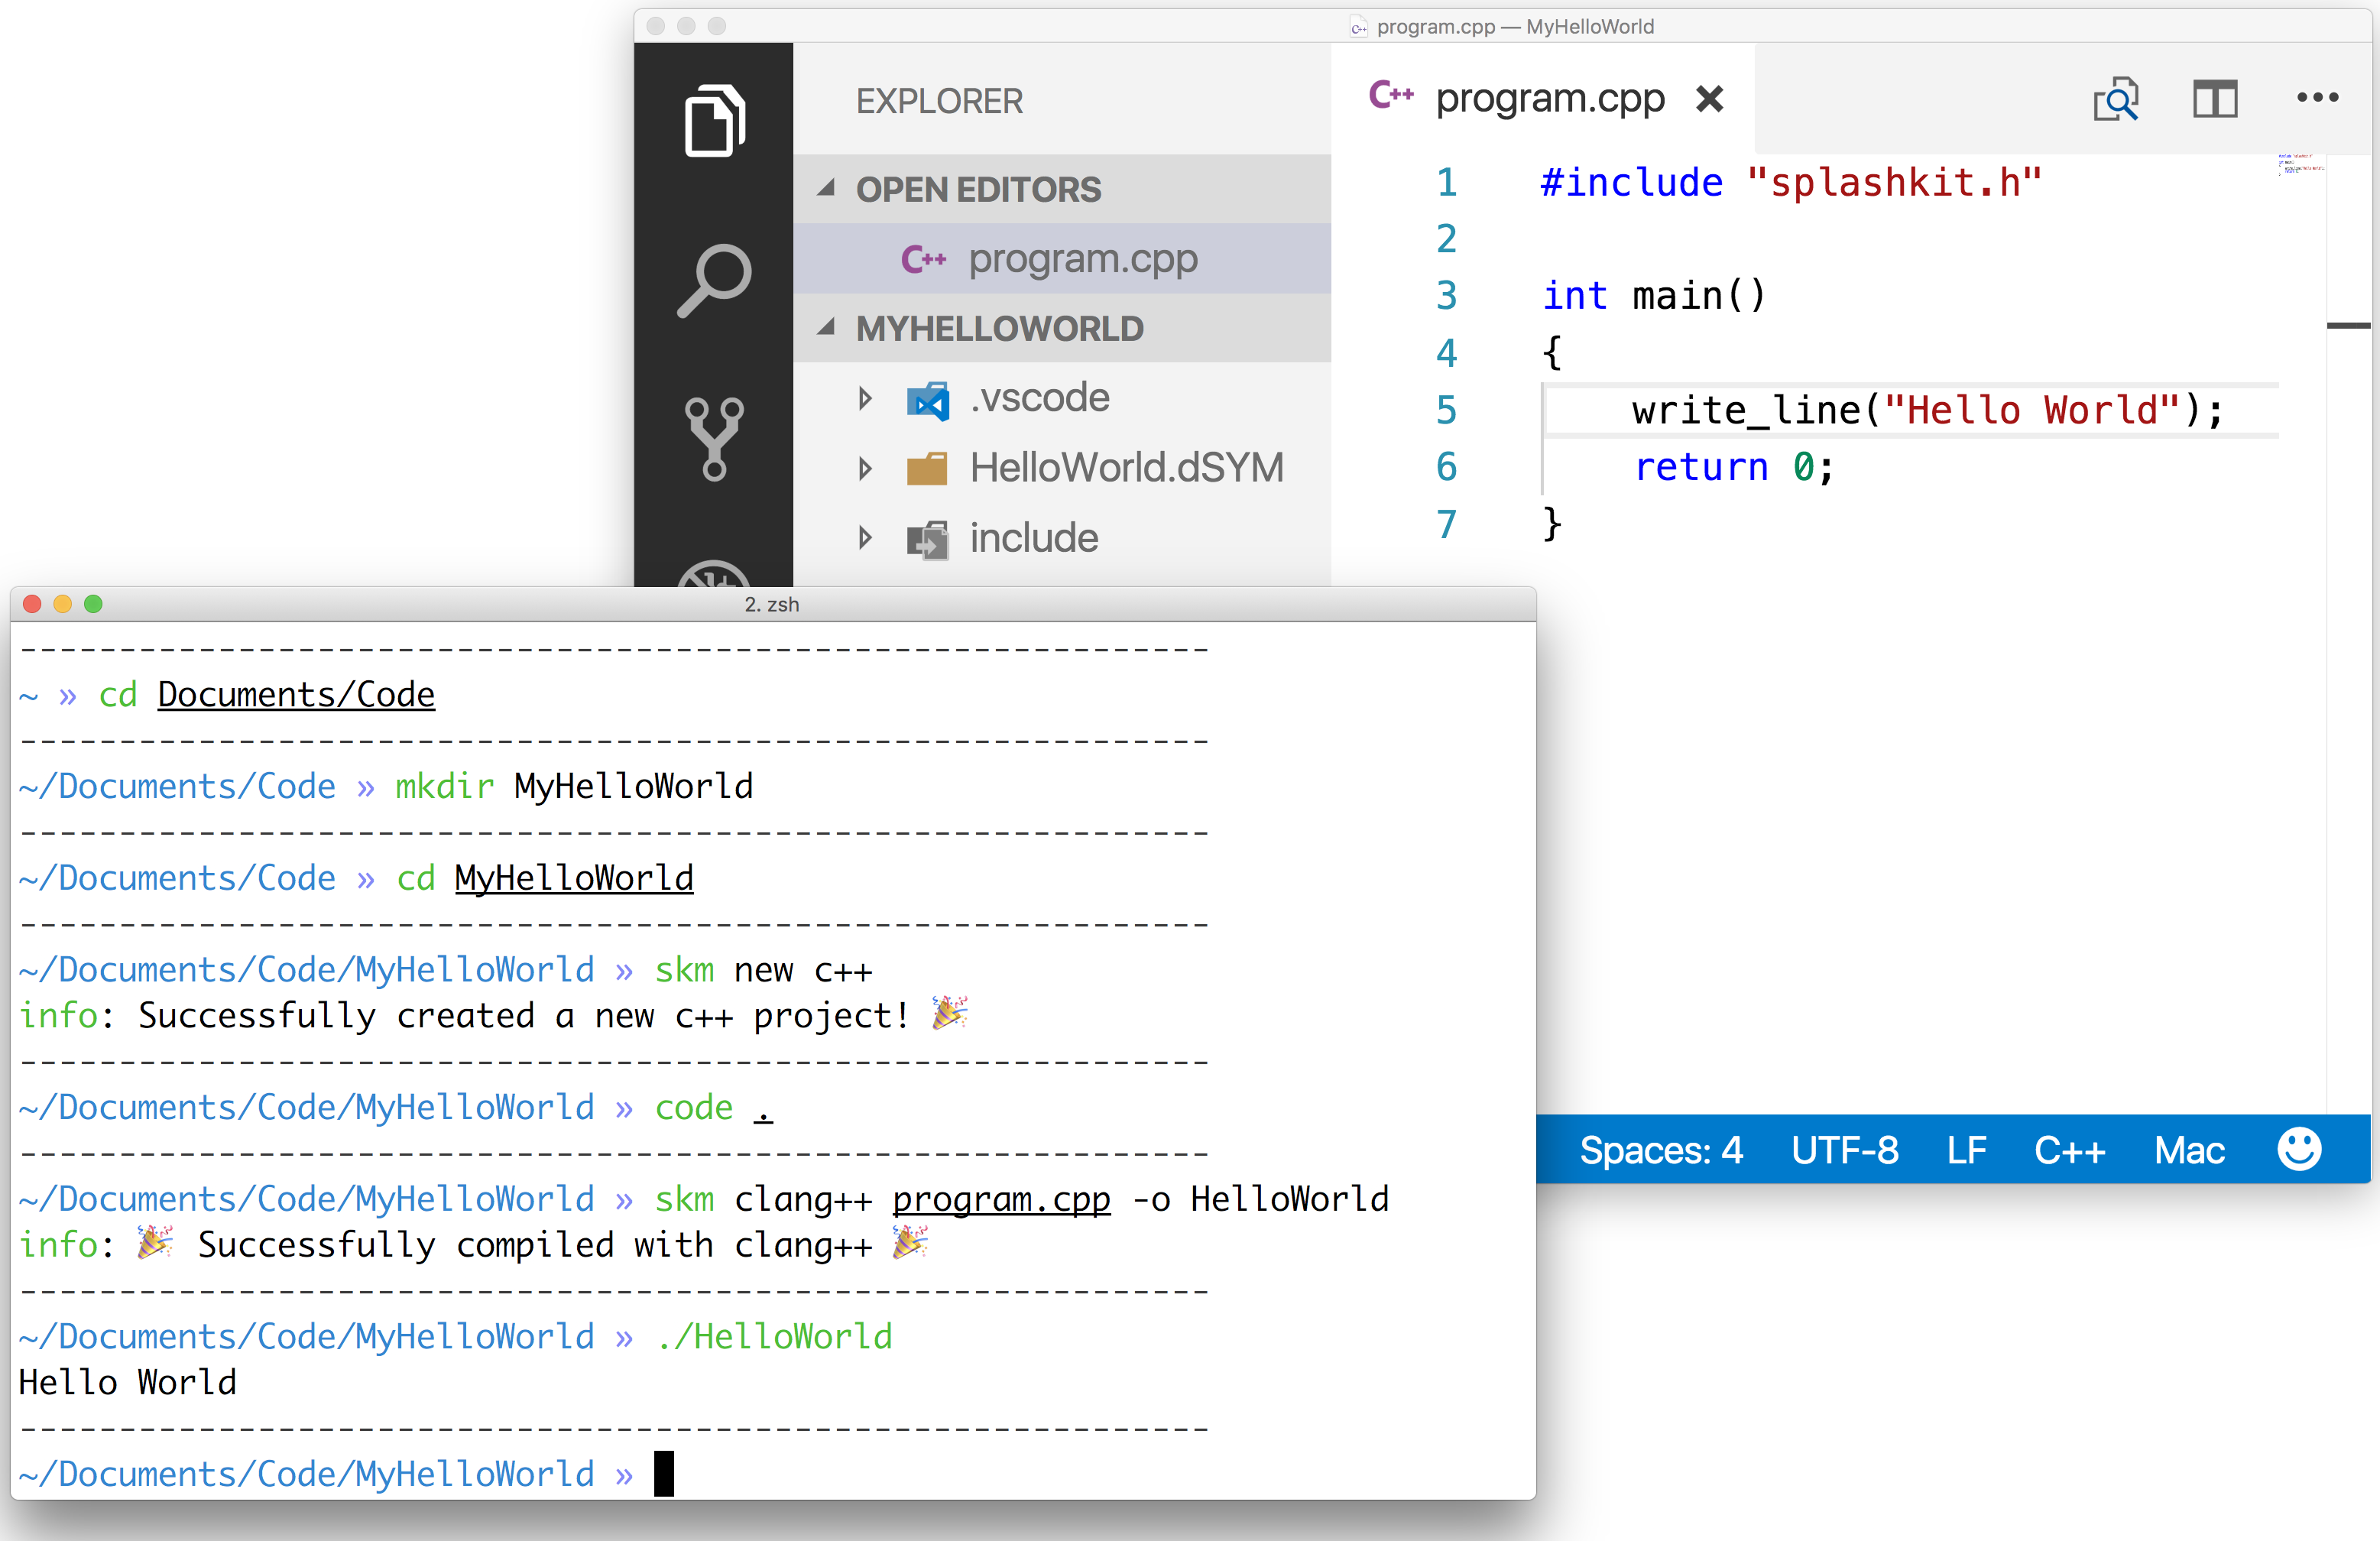
\includegraphics[width=0.8\textwidth]{./topics/programs-and-compilers/images/CppExample} 
   \caption{Editing and Compiling C++ code in Visual Studio Code}
   \label{fig:cpp-example}
\end{figure}

\fref{fig:fpc-example} shows the Hello World code in Visual Studio Code, which has a consistent look across all platforms. The figure also includes the command line instructions needed to setup a new SplashKit Pascal project, and compile it.

\begin{figure}[h]
   \centering
   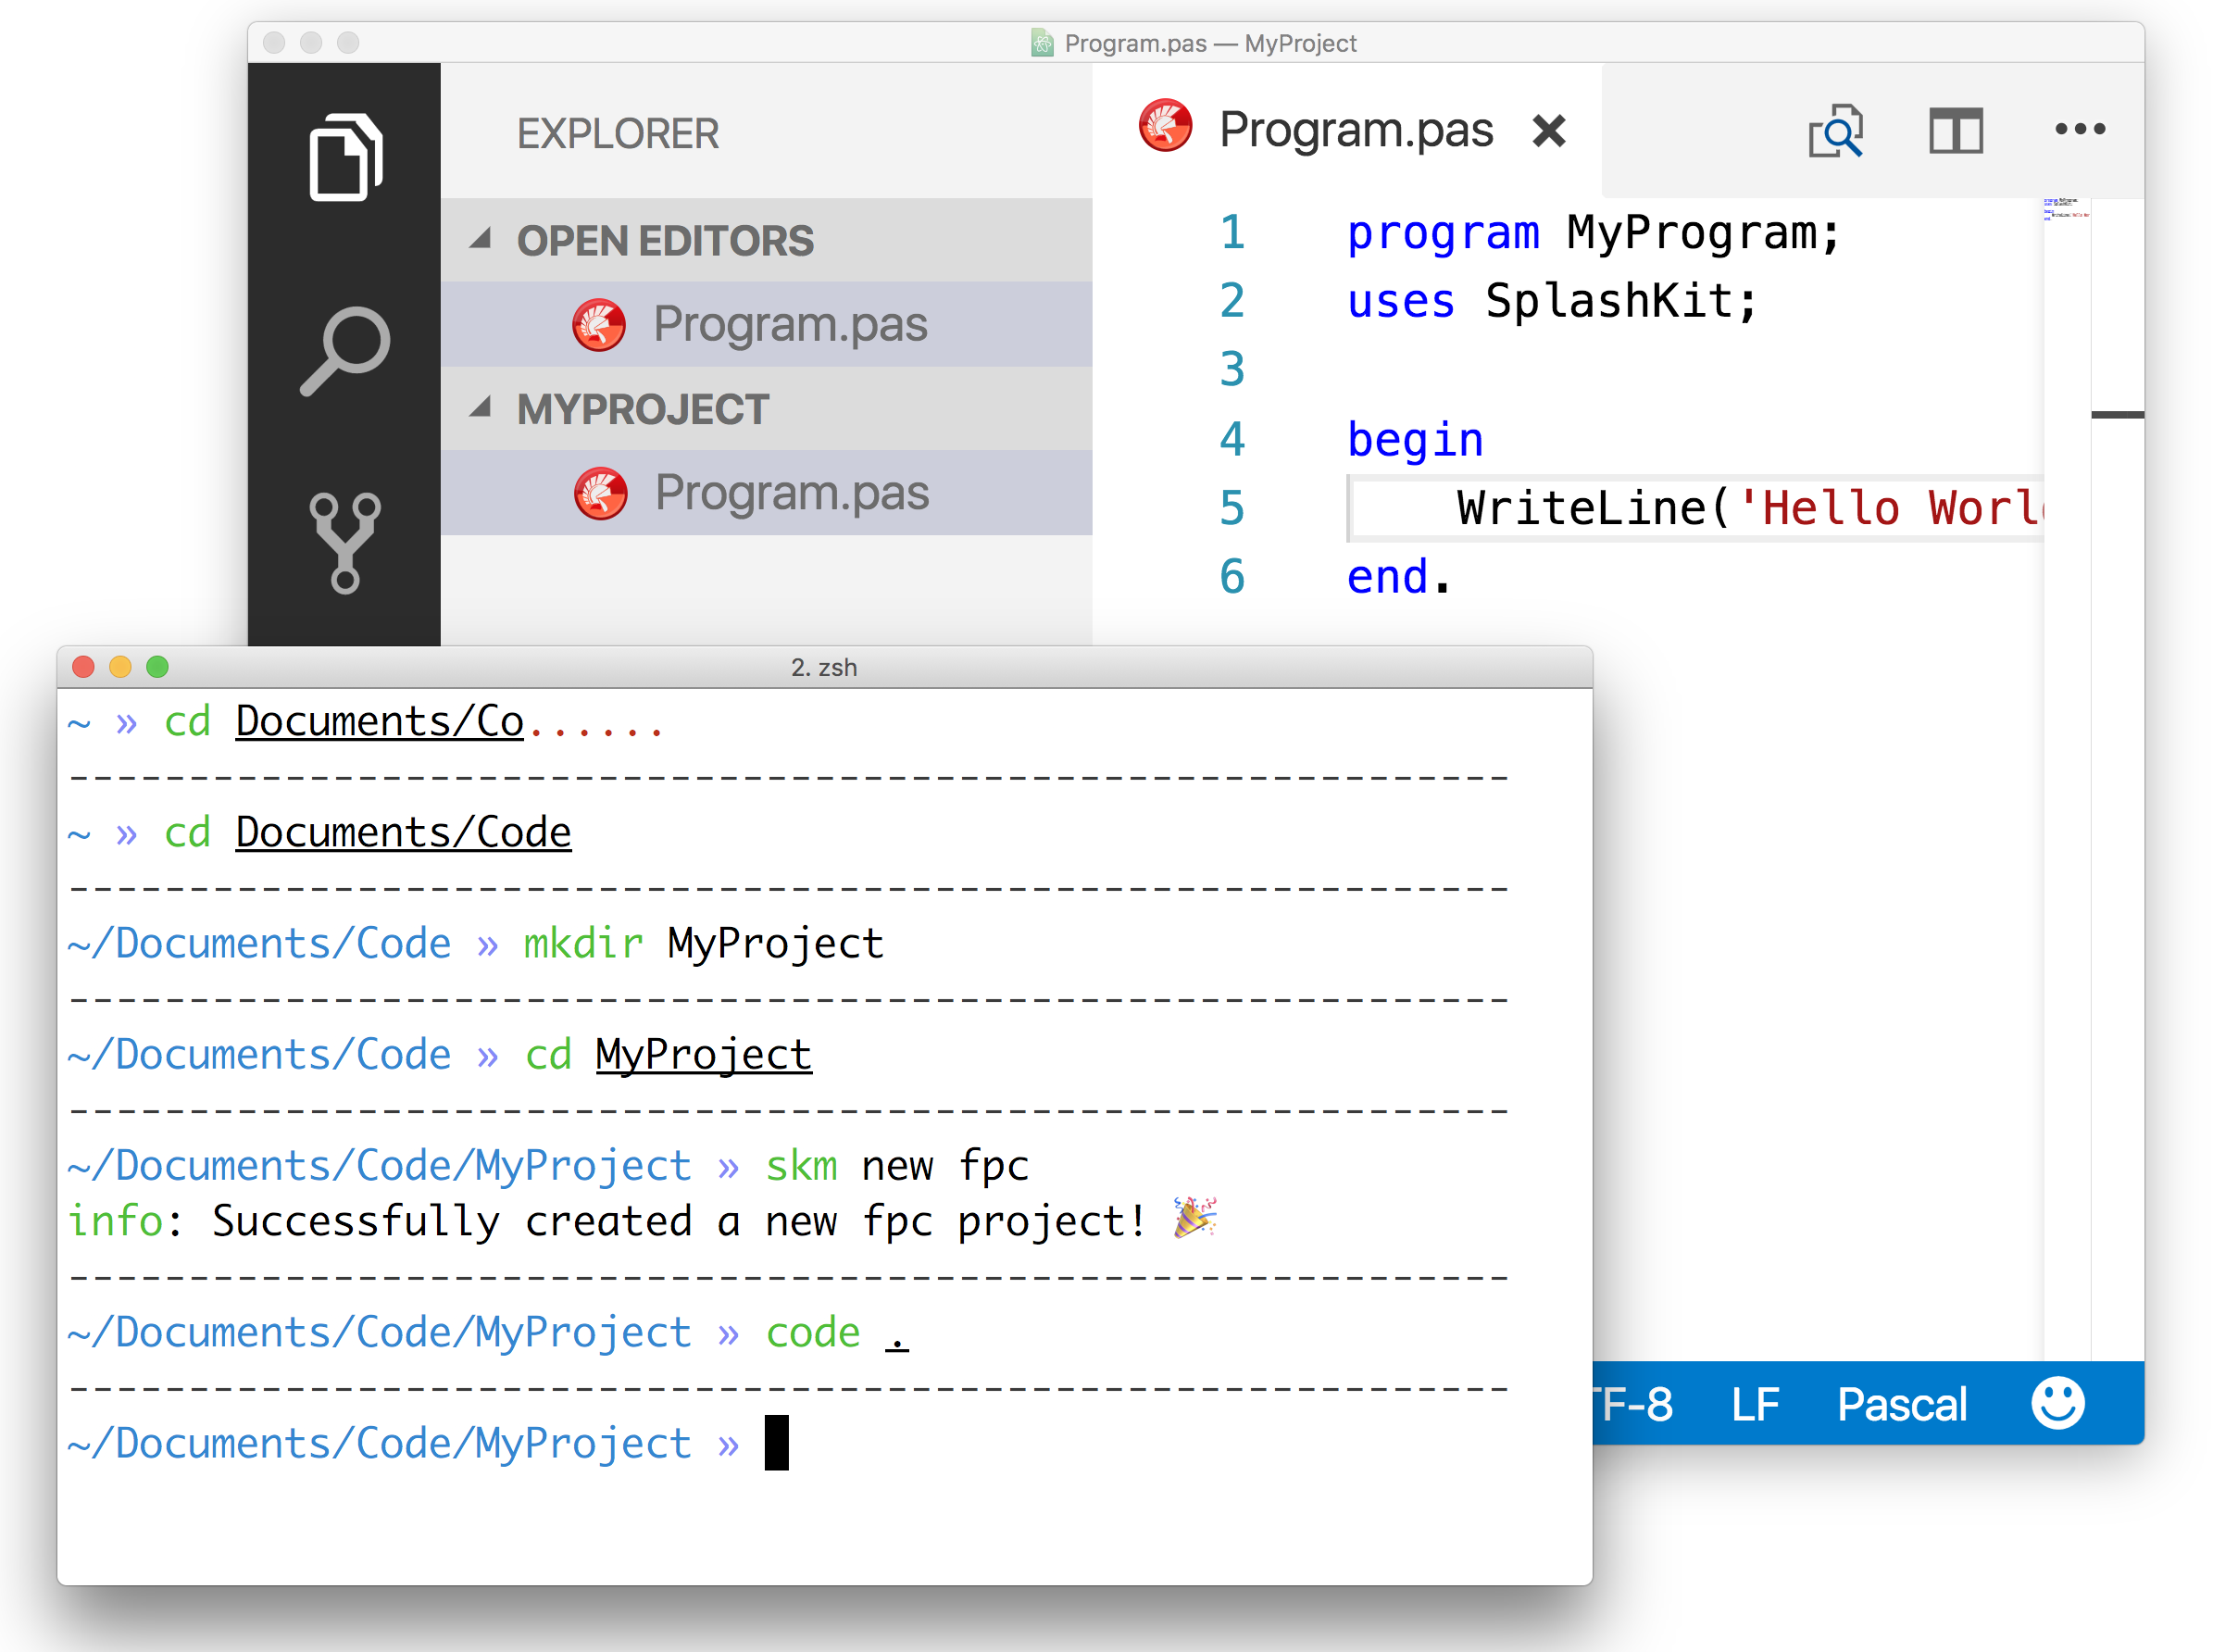
\includegraphics[width=0.8\textwidth]{./topics/programs-and-compilers/images/FpcExample} 
   \caption{Editing and Compiling Pascal code in Visual Studio Code}
   \label{fig:fpc-example}
\end{figure}

\clearpage
\subsubsection{Running the Compiler} % (fold)
\label{ssub:running_the_compiler}

Once you have saved the code to file it is time to compile your program. For this you are going to need to open a \nameref{sub:terminal}, and change into the directory where you saved the source code file. Once you are in this directory it is time to run the compiler.

When you run the compiler you need to give it two kinds of information: options, and the name of the file to compile. The compiler will read the code in the file you give it, and convert this to machine code as shown in \sref{sub:source_code_and_the_compiler} \nameref{sub:source_code_and_the_compiler}. The exact command you use depends on the compiler you are using.

\csection{
In C++ the compiler we will be using is called \textbf{clang++} (or \textbf{g++} the \textbf{GNU C++ Compiler}). The command you need to run in the Terminal is shown in Listing \ref{lst:compile-hello-world-c}. The \emph{-o name} option tells the compiler the name of the program file to create. In our example this will compile the code in \emph{hello-world.cpp} and save the machine code into a program called \emph{HelloWorld}.

\bashcode{lst:compile-hello-world-c}{Compiling C code.}{code/c/program-creation/compile-hello-world.sh}
}

\passection{
In Pascal the compiler we will be using is called \textbf{fpc}, which stands for the \textbf{Free Pascal Compiler}. The command you need to run in the Terminal is shown in Listing \ref{lst:compile-hello-world-pas}. The \emph{-S2} option is used to tell fpc to compile using the latest `Free Pascal' version of the language. In our example this will compile the code in \emph{HelloWorld.pas} and save the machine code into a program called \emph{HelloWorld}, which it gets from the name of the Pascal file.

\bashcode{lst:compile-hello-world-pas}{Compiling Pascal code.}{code/pascal/program-creation/compile-hello-world.sh}
}

Once you get the program to compile you can run it! This will load your program into memory, and start its steps running. The HelloWorld program will output the text `\texttt{Hello World!}' to the Terminal. To run the program you need to use its name. The command you need to enter is shown in \lref{lst:run-hello-world}, and in \fref{fig:run-helloworld}. The \texttt{./} before the file tells Bash to look in the current directory for the program.

\bashcode{lst:run-hello-world}{Bash command to run HelloWorld}{topics/programs-and-compilers/run-hello-world.sh}

\begin{figure}[h]
   \centering
   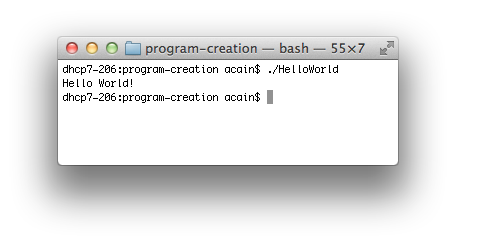
\includegraphics[width=0.7\textwidth]{./topics/programs-and-compilers/images/HelloWorld} 
   \caption[Hello World Terminal]{Hello World run from the Terminal}
   \label{fig:run-helloworld}
\end{figure}

% subsubsection running_the_compiler (end)

\subsubsection{When things do not work} % (fold)
\label{ssub:when_things_do_not_work}

Compilers are very specific about the code you give it. If the source code you try to compile does not follow all of the rules of the language then the compiler will fail, and end with an error message. These errors, called \textbf{syntax errors}, could be as small as missing a semicolon (;), or misspelling a name. To get your program to compile you will need to correct any syntax errors the compiler finds in your code.

\begin{figure}[h]
   \centering
   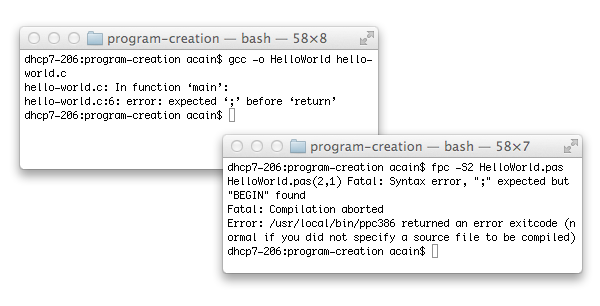
\includegraphics[width=0.8\textwidth]{./topics/programs-and-compilers/images/SyntaxErrors} 
   \caption{These Terminals show some syntax errors from programs that are missing a single semicolon (;)}
   \label{fig:syntax-errors}
\end{figure}

\fref{fig:syntax-errors} shows an example output caused by removing a single semicolon from the Hello World program's code. The numbers in the error messages give you an idea of where the compiler got to when it encountered the error. So the text \texttt{hello-world.c:6:} output from the C compiler indicates that the compiler got to line 6 before it encountered the error. The text \texttt{HelloWorld.pas(2,1)} output from the Pascal compiler indicates that it got up to line 2 character 1 before it encountered the error.

When the compiler encounters these issues it does not create the executable program. You need to learn to use these error messages to help you locate errors in your code, so that you can fix them, and then run the compiler again to generate your program.

\mynote{
\begin{itemize}
  \item Syntax errors are very common. Do not worry when this occurs to you.
  \item Always start with the first error. The compiler will try to continue compiling your code after it finds an error. This can mean that later errors do not really exist, once you fix the earlier ones.
  \item Unfortunately compiler error messages are not always very clear on what the cause of the error is. You need to learn how to read and understand these messages.
  \item To get good at programming requires lots of practice.
\end{itemize}
}

% subsubsection when_things_do_not_work (end)



% section the_compiler (end)


% section using_these_concepts_compiling_a_program (end)


\clearpage
\def\pageLang{none}
\section{Installing a Text Editor} % (fold)
\label{sec:installing_a_text_editor}

When you are programming you will spend most of your time in a Text Editor. The best kinds of editors for program code include \emph{syntax highlighting} where the editor uses details about the language to highlight parts of the code as you write it. This can make it easier to find and fix small errors as you go.

There are many different syntax highlighting text editors, each will support different programming languages and operating systems. The following text editors support the C and Pascal programming languages. Install the one appropriate for your operating system.

\begin{itemize}
  \item \nameref{ssub:gedit_on_linux}
  \item \nameref{ssub:textwrangler_or_textmate_on_mac_os}
  \item \nameref{ssub:notepad_for_windows}
\end{itemize}

\subsubsection{gEdit on Linux} % (fold)
\label{ssub:gedit_on_linux}

The \textbf{gEdit} program is a syntax highlighting text editor for Linux. In Ubuntu this is the standard \textbf{Text Editor} program found in \emph{Accessories}. This will come as part of the operating system installation, so you do not need to install a separate editor. 

% subsubsection gedit_on_linux (end)

\subsubsection{TextWrangler on Mac OS} % (fold)
\label{ssub:textwrangler_or_textmate_on_mac_os}

TextWrangler is a free syntax highlighting text editor for Mac OS. You can download and install this from the \textbf{Mac App Store}, or from their web site.

\begin{itemize}
  \item Mac App Store link: \url{http://itunes.apple.com/au/app/textwrangler/id404010395?mt=12}
  \item Website: \url{http://www.barebones.com/products/textwrangler/}
  \item TextMate is another good editor, though it is not free: \url{http://macromates.com/}
\end{itemize}

% subsubsection textwrangler_or_textmate_on_mac_os (end)

\subsubsection{Notepad++ on Windows} % (fold)
\label{ssub:notepad_for_windows}

Notepad++ is a free syntax highlighting text editor for Windows. You can download and install this from the Notepad++ website.

\begin{itemize}
  \item Notepad++: \url{http://notepad-plus-plus.org/}
\end{itemize}

% subsubsection notepad_for_windows (end)

% subsection installing_a_text_editor (end)
% =============
% = C Section =
% =============
\clearpage
\def\pageLang{c}
\section{Using the C++ Compiler} % (fold)
\label{sec:building_programs_in_c}

The C++ programming language is very powerful and flexible. In this section you will see the tools that you need to start programming with C++ on your computer.

\clearpage
\subsection{Hello World in C} % (fold)
\label{sub:hello_world_in_c}

Now that you have the compiler installed you can create your first program: the famous \textbf{Hello World} discussed in \sref{sub:hello world}. The C code for this is shown in \lref{lst:hello-world-c-c}. This code tells the computer to `print' the text \emph{Hello World!} to the Terminal. Do the following to create this program for yourself, see the notes below for hints:

\begin{enumerate}
  \item Open your text editor
  \item Create a new text file
  \item Type\footnote{Do not just copy and paste it out of the text, type it in yourself as this will help you learn the concepts being covered.} in the text below, making sure you get every character correct.
  \item Save your program's code in a file called \textbf{hello-world.c}, and note the directory where it is saved
  \item Open the Terminal
  \item Change into the directory where you save the file
  \item Compile the program using \texttt{gcc -o HelloWorld hello-world.c}
  \item Run the program using \texttt{./HelloWorld}
\end{enumerate}

Well done, you have now created and run your first C program!

\csection
{
\ccode{lst:hello-world-c-c}{Hello World code in C.}{code/c/program-creation/hello-world.c}
}

\mynote{
\begin{itemize}
  \item See \sref{sec:installing_a_text_editor} \nameref{sec:installing_a_text_editor} for details on installing the Text Editor.
  \item See \nameref{ssub:bash} in \sref{sub:terminal} for an example of how to use the Terminal.
  \item See \sref{sec:using_these_concepts_compiling_a_program} \nameref{sec:using_these_concepts_compiling_a_program} for the overall process and the output you should expect from the program.
\end{itemize}
}

% subsection hello_world_in_c (end)

\clearpage
\def\pageLang{pas}
\section{Installing and Using the Pascal Compiler} % (fold)
\label{sec:the_pascal_compiler}

The Pascal language is a great first programming language. It is both powerful and clear in its syntax. In this section you will see the tools that you 

\mynote{
If you are using C you do not need to install the Pascal compiler, instead you should read \sref{sec:building_programs_in_c} \nameref{sec:building_programs_in_c}.
}

\subsection{Installing the Free Pascal Compiler} % (fold)
\label{sub:installing_fpc}

You can get the Free Pascal Compiler (fpc) for Linux, Mac OS, and Windows. The following section describe where it is you can find these programs, and how to install them.

\subsubsection{Installing fpc on Linux} % (fold)
\label{ssub:fpc_linux}

It should be relatively easy to install \textbf{fpc} for Linux. To install this on Ubuntu linux use the command shown in \lref{lst:apt-get-fpc}.

\bashcode{lst:apt-get-fpc}{The command line instruction to install fpc on Ubuntu}{topics/programs-and-compilers/pascal/apt-get-fpc.txt}

% subsubsection linux (end)

\subsubsection{Installing fpc on Mac OS} % (fold)
\label{ssub:installing_gcc_on_mac_os}

To install \textbf{fpc} on Mac OS you need to install the \textbf{XCode} developer tools, and then the \textbf{Free Pascal Compiler}. You can get the latest version of XCode from the \textbf{Mac App Store}, and then download and install the Free Pascal Compiler from their website.

\begin{itemize}
  \item XCode links:
  \begin{itemize}
    \item Apple's XCode website \url{http://developer.apple.com/xcode/}
    \item Mac App Store  \url{http://itunes.apple.com/au/app/xcode/id448457090?mt=12}
    \item For older version of Mac OS, download from \href{https://developer.apple.com/downloads/download.action?path=Developer_Tools/xcode_3.2.2_developer_tools_beta_20728/xcode322_2148_developerdvd.dmg}{Apple's developer site}.\footnote{These will require you to have an Apple Developer account, which can be done for free at \url{http://developer.apple.com/programs/register}.}
  \end{itemize}
  \item Free Pascal links:
  \begin{itemize}
    \item The Free Pascal Website \url{http://freepascal.org}
    \item Download the compiler from \url{http://sourceforge.net/projects/freepascal/files/} 
  \end{itemize}
\end{itemize}

% subsubsection installing_gcc_on_mac_os (end)

\subsubsection{Installing gcc on Windows} % (fold)
\label{ssub:installing_gcc_on_windows}

To install \textbf{fpc} on Windows you need to install the \textbf{MinGW} program and the \textbf{Free Pascal Compiler}. This includes the MinGW Shell, the Terminal equivalent for Windows. Read the Getting Started page from the links below, and follow the steps for the \textbf{Graphical User Interface Installer}. When following the installer make sure that you choose to install the MinGW Shell as well as the C and C++ compilers.

\begin{itemize}
  \item MinGW:
  \begin{itemize}
    \item The project's Website \url{www.mingw.org}
    \item Instructions for installing MinGW: \url{http://www.mingw.org/wiki/Getting_Started}
    \item Follow the link from the Getting Started article, or download MinGW from Source Forge at \url{http://sourceforge.net/projects/mingw/}
    \item It is a good idea to restart after installing MinGW to make sure all its settings are applied.
  \end{itemize}

  \item Free Pascal links:
  \begin{itemize}
    \item The Free Pascal Website \url{http://freepascal.org}
    \item Download the compiler from \url{http://sourceforge.net/projects/freepascal/files/} 
  \end{itemize}
  
\end{itemize}



% subsubsection installing_gcc_on_windows (end)
% \clearpage
\subsubsection{Testing fpc has installed} % (fold)
\label{ssub:testing_your_install_fpc}

To test that you have successfully installed gcc you can do the following:
\begin{enumerate}
  \item Open a Terminal window. (See the notes on the \nameref{sub:terminal} page for the location of the Terminal program)
  \item At the terminal type \textbf{\texttt{fpc}}. You should see something similar to \fref{fig:fpc-install}. If you see the message `\texttt{-bash: fpc: command not found}' this means the install has not worked correctly. Please review the install steps for your Operating System or get someone to check your install.
\end{enumerate}

\begin{figure}[h]
   \centering
   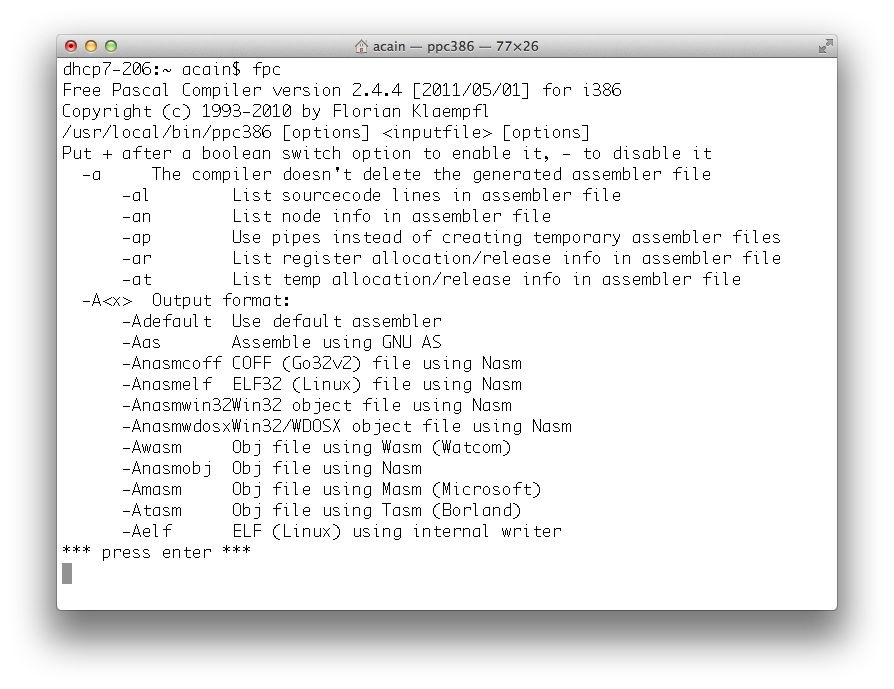
\includegraphics[width=\textwidth]{./topics/programs-and-compilers/images/fpcInstall} 
   \caption{Testing fpc has been installed}
   \label{fig:fpc-install}
\end{figure}

% subsection testing_your_install (end)

% subsection installing_gcc (end)
\subsection{Hello World in Pascal} % (fold)
\label{sub:hello_world_in_pascal}

Now that you have the compiler installed you can create your first program: the famous \textbf{Hello World} discussed in \sref{sub:hello world}. The Pascal code for this is shown in \lref{lst:hello-world-pas-pas}. This code tells the computer to `write' the text \emph{Hello World!} to the Terminal. Do the following to create this program for yourself, see the notes below for hints:

\begin{enumerate}
  \item Open a Terminal
  \item Navigate to where you want to save your code, and create a new folder using \texttt{mkdir} and the project name (without spaces).
  \item Move into the project folder using the \texttt{cd} command.
  \item Use \texttt{skm} to create a new Pascal project.
  \item Open Visual Studio Code, and open the \textbf{folder} that contains your project code.
  \item Type\footnote{Do not just copy and paste it out of the text, type it in yourself as this will help you learn the concepts being covered.} in the text below, making sure you get every character correct.
  \item Compile the program using \texttt{skm fpc -S2 program.pas}
  \item Run the program using \texttt{./HelloWorld}
\end{enumerate}

Well done, you have now created and run your first Pascal program!

\passection
{
\pascode{lst:hello-world-pas-pas}{Hello World code in Pascal.}{code/pascal/program-creation/HelloWorld.pas}
}

\mynote{
\begin{itemize}
  \item See \sref{subs:install} \nameref{subs:install} for details on installing the tools you need.
  \item See \nameref{ssub:bash} in \sref{sub:terminal} for an example of how to use the Terminal.
  \item See \sref{sec:using_these_concepts_compiling_a_program} \nameref{sec:using_these_concepts_compiling_a_program} for the overall process and the output you should expect from the program.
\end{itemize}
}

% subsection hello_world_in_c (end)


% section the_pascal_compiler (end)
\clearpage
\def\pageLang{none}
\section{Graphical Applications with SwinGame} % (fold)
\label{sub:graphical_applications_with_swingame}

SwinGame is a 2D game creation library. It contains a number of resources that you can use to create small games using the C and Pascal. To get started with SwinGame you need to download a \emph{template} from the website. The template includes everything you need to get started creating a game in SwinGame.

\subsubsection{Installing SwinGame} % (fold)
\label{ssub:installing_swingame}

The good news is that SwinGame does not require you to install anything on Mac OS or Windows. On Linux you will need to install some libraries, and compile the SwinGame library. The instructions for this are on the SwinGame web site: \url{http://www.swingame.com/wiki/index.php/SwinGame_3_Beta}.

The SwinGame templates contain a project template. This includes the SwinGame library, scripts to build your program, and some basic resources (images, sounds, fonts) used in the SwinGame splash screen.

\begin{figure}[h]
   \centering
   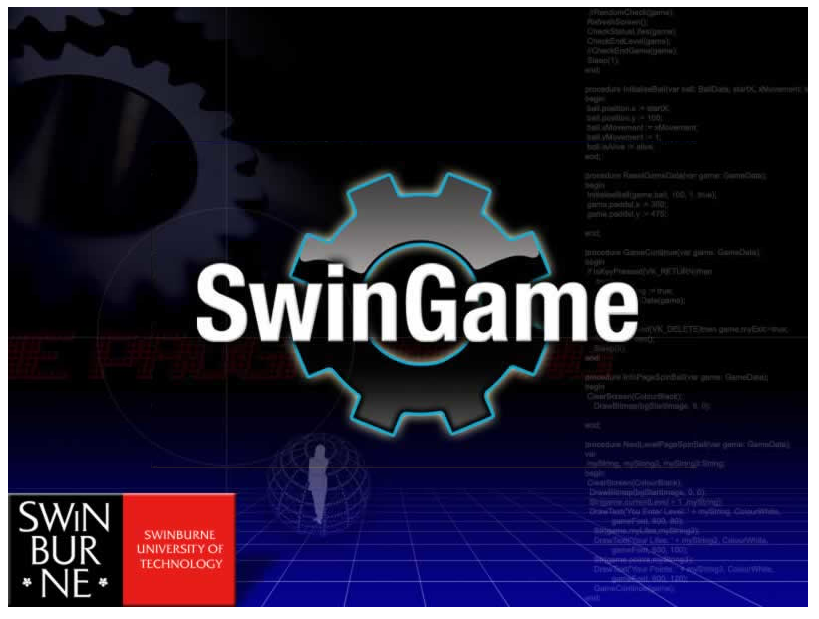
\includegraphics[width=0.5\textwidth]{./topics/programs-and-compilers/images/SwinGameSplash} 
   \caption{SwinGame splash screen}
   \label{fig:swingame-splash}
\end{figure}

\begin{figure}[h]
   \centering
   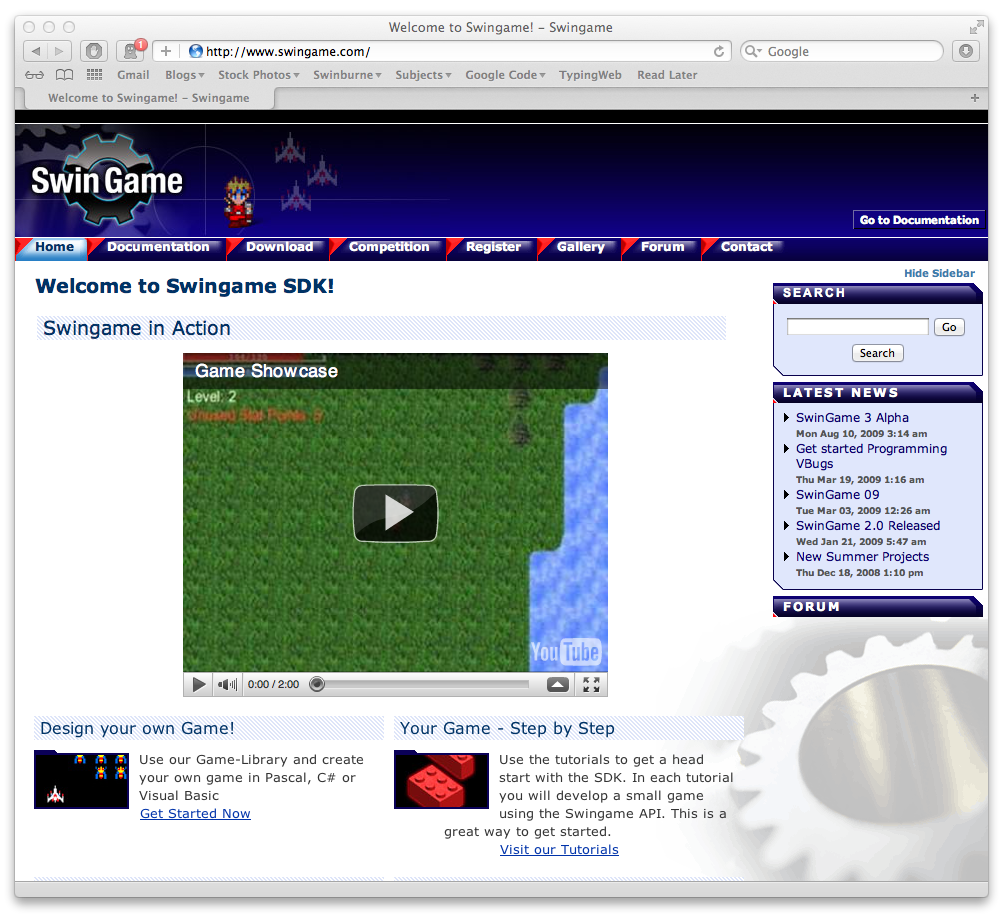
\includegraphics[width=0.5\textwidth]{./topics/programs-and-compilers/images/SwinGameSite} 
   \caption{SwinGame website}
   \label{fig:swingame-site}
\end{figure}


% subsubsection installing_swingame (end)

\clearpage
\subsubsection{Coding a SwinGame} % (fold)
\label{ssub:coding_a_swingame}

The SwinGame project template contains a number of directories to organise your projects code and resources. Within the project directory itself you will find the following files and directories:

\begin{itemize}
  \item \textbf{bin}: When you compile your game it will be placed into this directory. The name \emph{bin} indicates that this contains the \emph{binary} version of the program, the one that contains the \nameref{sub:machine_code}.
  \item \textbf{build.sh}: This file contains a Bash script that will compile your project for you. When you run this script it will compile the code in the \emph{src} directory, and place the resulting game with its resources in the \emph{bin} directory.
  \item \textbf{clean.sh}: This file contains another Bash script, this one cleans up the binary and temporary files the \emph{build.sh} script creates.
  \item \textbf{lib}: Contains the libraries used by SwinGame. This includes the C code used to access these libraries which you can browse if you are interested in seeing what code is available to you.
  \item \textbf{Resources}: This directory contains the resources used by your game. This includes images, sounds, fonts, and other resources. When you want to use your own resources they will need to be placed under this directory in the appropriate subdirectory.
  \item \textbf{run.sh}: This third Bash script contains the instructions to run your program. This is provided for convenience.
  \item \textbf{src}: Is the directory that will contain your game's code. The standard template contains a basic template you can use to get started.
  \item \textbf{tmp}: Stores temporary files created by the compiler. 
\end{itemize}

To start experimenting with SwinGame, you should download a new project and compile it. The following steps outline how to do this:
\begin{enumerate}
  \item \textbf{Download} the version of SwinGame for your programming language and Operating System (You can download this from \url{http://www.swingame.com/wiki/index.php/SwinGame_3_Beta}). 
  \item \textbf{Extract} the \emph{Project Template} from the file you downloaded.
  \item \textbf{Rename} the directory to the name of your game, call the first one \textbf{HelloWorld}.
  \item \textbf{Open} a \nameref{sub:terminal}, and \emph{change directory} so that you are in your game directory, inside the \emph{HelloWorld} directory, if that is what you called your game.
  \item \textbf{Compile} the program by running the \emph{build.sh} script. You do this by typing \texttt{./build.sh} and pressing enter.
  \item \textbf{Execute} the program by running the \emph{run.sh} script to run your game. You can do this by typing \texttt{./run.sh} and pressing enter. Alternatively you can find the game in the \texttt{bin} directory, where it can be run by double clicking.
\end{enumerate}

Once you have this compiling and running you can start to play with the source code. The code for your SwinGame can be found in the \textbf{\texttt{src}} folder. This includes a \texttt{\textbf{main.c}} file, where you can place your source code.

% subsubsection coding_a_swingame (end)

% subsection graphical_applications_with_swingame (end)


% section building_programs_in_c (end)

% ===================================
% = Understanding Building Programs =
% ===================================

\clearpage
\def\pageLang{}
\section{Understanding Program Compilation} % (fold)
\label{sec:understanding_program_compilation}

An in depth look at how programs and compilers work is beyond the scope of this book. Instead, this chapter focuses on two aspects that can help you understand why we need compilers, and how these are able to help us. These topics are \nameref{sub:levels_of_abstraction}, followed by \nameref{sub:computers_and_intelligent_behaviour}.

\subsection{Levels of Abstraction} % (fold)
\label{sub:levels_of_abstraction}

Programs are very complicated. Trying to keep all of the details about how it works in focus all of the time would take a large amount of effort, and slow you down. As humans we have developed strategies for dealing with these kinds of situations. What we do is create \emph{layers} of abstraction.

A layer, or level, of abstraction provides a means of managing details at a similar level of detail. This means that all aspects of that level are similar, and related to each other. When you are working at a certain level, you think in terms of the tools and artefacts that are available to you. 

These levels build on top of each other, with each layer being built on top of the lower layer, and providing the foundation for the next higher layer. Within a layer of abstraction you do not need to think about the lower levels of abstraction, most of the time. However, it is always good to know the details of at least one level of abstraction below the level you are working at.

\subsubsection{Programming Abstraction Levels} % (fold)
\label{ssub:programming_abstraction_levels}

Computers are unintelligent. This is one of the first, and most important, things you need to understand when starting to create your own programs. A computer is a machine that can be programmed using \nameref{sub:machine_code}. These binary commands instruct the computer to perform basic actions such as adding numbers, reading values from memory, storing values in memory, jumping to new instructions elsewhere in memory, and other simple tasks. While this is a very low level, it is not the lowest level of abstraction.

Below machine code, there is the abstraction for \textbf{binary}. This is the idea that you can have a number system based on two digits, 0 and 1. The machine code level builds on this idea, creating a set of instructions that can be used to tell the computer what to do. Below binary there is the concept of \textbf{gates}, which are themselves built on top of \textbf{electronic circuits}, which in turn are made from \textbf{discrete electronic components}. Even these low level electronic components are based upon something else, but to discuss this we would need to delve into the realm of \textbf{semiconductors} and \textbf{Quantum Mechanics}. From machine code you can also work up to \nameref{sub:assembly}, and then to \nameref{sub:source_code_and_the_compiler}.

Whenever you are working on something you need to be able to work at that level of abstraction, and have an understanding of the level below, and the level above. For programming this means that you will need to understand of the tools provided to you by the language (a level below), and you need to understand the features and functions of the program you are creating (a level above).

In this book the \emph{Understanding} section of each chapter will help you see how the concepts covered work at a lower level of abstraction. Often this means these sections are very detailed. You should read these sections to understand how the abstractions (concepts) covered in the chapter work, at a level of abstraction lower than you will be working at.

% subsubsection programming_abstraction_levels (end)
% subsection levels_of_abstraction (end)
\clearpage
\subsection{Computers and Intelligent Behaviour} % (fold)
\label{sub:computers_and_intelligent_behaviour}

If computers are unintelligent, how can they do the awesome things they do?

That is a good question. Computers are unintelligent, but programs are not. The computer does not \emph{know} what it is doing. It is following a set of steps that was coded into the program being executed. These steps, however, were created by people, software developers. When a computer does something cool, its because a person told it to do that.

This is why it can be really great fun to be a software developer. You get to make computers do things you want them to. This creativity can be really exhilarating when you finally get your program to do exactly what you want.

\begin{figure}[h]
   \centering
   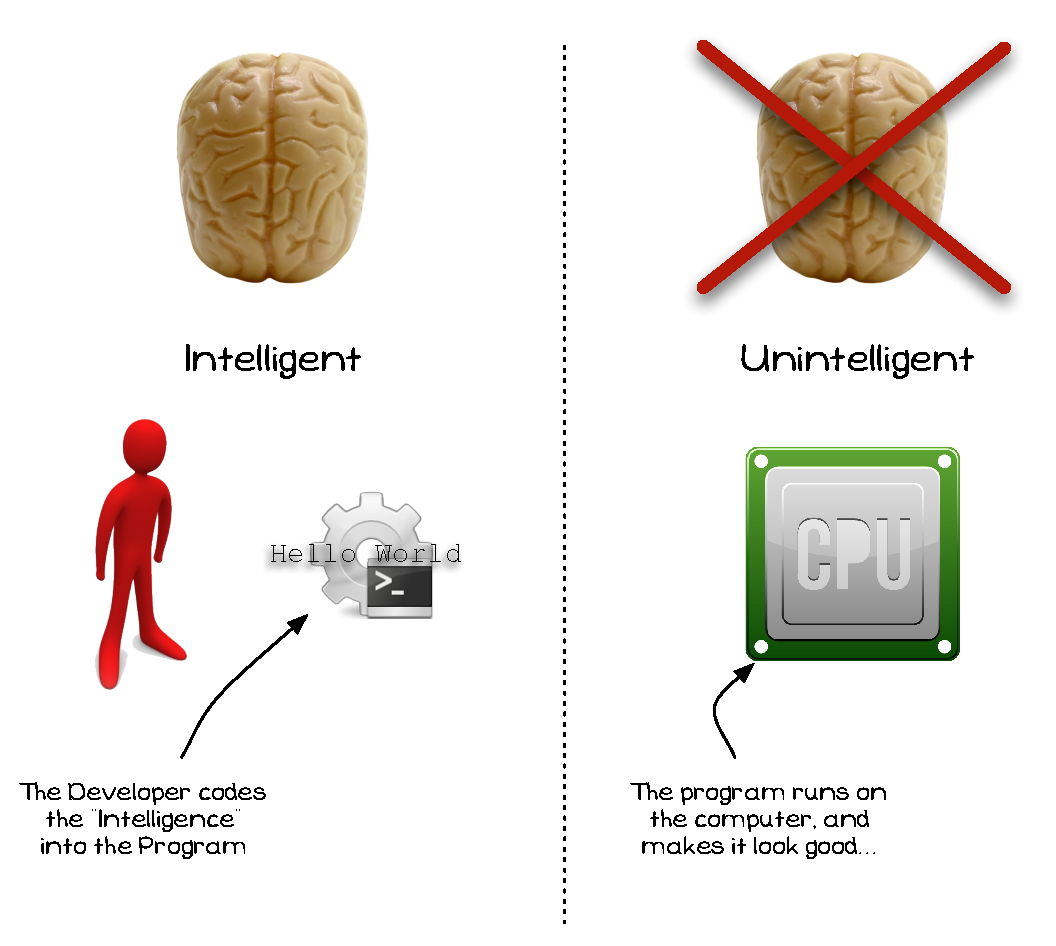
\includegraphics[width=\textwidth]{./topics/programs-and-compilers/diagrams/ProgramIntelligence} 
   \caption{Computers are unintelligent, any interesting behaviour comes from programs created by software developers}
   \label{fig:program-intelligence}
\end{figure}
% subsection computers_and_intelligent_behaviour (end)
% section understanding_ (end)

% ============
% = Examples =
% ============

\clearpage
\section{Exercises on Building Programs} % (fold)
\label{sec:examples_and_exercises_on_building_programs}

\subsection{Concept Questions} % (fold)
\label{sub:concept_questions_compiler}

Read over the concepts in this chapter and answer the following questions:
\begin{enumerate}
  \item What is a \nameref{sub:what_is_a_program_}? What does it contain?
  \item What is \nameref{sub:machine_code}?
  \item Can you write programs in Machine Code? Explain any issues associated with this.
  \item What is \nameref{sub:assembly}?
  \item Can you write programs in Assembly? Explain any issues associated with this.
  \item What tool is used to convert Assembly to Machine Code?
  \item What is Source Code?
  \item What are the advantages of programming at a Source Code level?
  \item What tool is used to convert Source Code to Machine Code?
  \item Why do you need to convert Source Code and Assembly to Machine Code?
  \item What is the \nameref{sub:terminal}? 
  \item What is Bash?
  \item Which command is used to change directories in Bash?
  \item With Bash, how can you check which directory is the current working directory?
  \item How can you list all of the files in the current directory?
  \item Why program `Hello World'? What does it do for you?
  \item What is the name of the C or Pascal compiler we will be using in this book?
  \item How intelligent is your computer?
\end{enumerate}
% subsection concept_questions (end)

\medskip
\subsection{Code Writing Questions: Applying what you have learnt} % (fold)
\label{sub:code_writing_questions_applying_what_you_have_learnt_compiler}

Apply what you have learnt to the following tasks:

\begin{enumerate}
  \item Install the following programs:
  \begin{enumerate}
    \item A \textbf{Text Editor} that offers syntax highlighting for the language you are using.
    \item The \textbf{Compiler} for the language you are using.
    \item \textbf{Bash} and the \textbf{Terminal} (on Windows only).
  \end{enumerate}
  \item Enter the code, compile, and run the `Hello World' program.
  \item Try changing the code to output a different message. After you have made the changes you will need to re-compile and run the program.
\end{enumerate}
% subsection code_writing_questions_applying_what_you_have_learnt (end)

\clearpage
\subsection{Extension Questions} % (fold)
\label{sub:extension_questions_compiler}

If you want to further your knowledge in this area you can try to answer the following questions. The answers to these questions will require you to think harder, and possibly look at other sources of information.
\begin{enumerate}
  \item What is the difference between a compiler and an interpreter? How are programs of interpreted languages, such as Python, executed?
  \item If you compile a program for an Intel CPU on UNIX, can you run this on a UNIX machine that has a PowerPC CPU?
  \item If you compile a program on a Windows machine can you run the resulting program on a UNIX machine with the same CPU architecture?
  \item What is a fat, or Universal, binary?
  \item What is a Virtual Machine?
\end{enumerate}
% subsection extension_questions (end)
% section examples_and_exercises_on_building_programs (end)


% chapter building_programs (end)